% Generated by Sphinx.
\def\sphinxdocclass{report}
\documentclass[letterpaper,10pt]{sphinxmanual}
\usepackage[utf8]{inputenc}
\DeclareUnicodeCharacter{00A0}{\nobreakspace}
\usepackage{cmap}
\usepackage[T1]{fontenc}
\usepackage{babel}
\usepackage{times}
\usepackage[Sonny]{fncychap}
\usepackage{longtable}
\usepackage{sphinx}
\usepackage{multirow}


\title{星际移民之书}
\date{2015 年 01 月 23 日}
\release{3.14}
\author{Interplanetary Immigration Center}
\newcommand{\sphinxlogo}{}
\renewcommand{\releasename}{发布}
\makeindex

\makeatletter
\def\PYG@reset{\let\PYG@it=\relax \let\PYG@bf=\relax%
    \let\PYG@ul=\relax \let\PYG@tc=\relax%
    \let\PYG@bc=\relax \let\PYG@ff=\relax}
\def\PYG@tok#1{\csname PYG@tok@#1\endcsname}
\def\PYG@toks#1+{\ifx\relax#1\empty\else%
    \PYG@tok{#1}\expandafter\PYG@toks\fi}
\def\PYG@do#1{\PYG@bc{\PYG@tc{\PYG@ul{%
    \PYG@it{\PYG@bf{\PYG@ff{#1}}}}}}}
\def\PYG#1#2{\PYG@reset\PYG@toks#1+\relax+\PYG@do{#2}}

\expandafter\def\csname PYG@tok@gd\endcsname{\def\PYG@tc##1{\textcolor[rgb]{0.63,0.00,0.00}{##1}}}
\expandafter\def\csname PYG@tok@gu\endcsname{\let\PYG@bf=\textbf\def\PYG@tc##1{\textcolor[rgb]{0.50,0.00,0.50}{##1}}}
\expandafter\def\csname PYG@tok@gt\endcsname{\def\PYG@tc##1{\textcolor[rgb]{0.00,0.27,0.87}{##1}}}
\expandafter\def\csname PYG@tok@gs\endcsname{\let\PYG@bf=\textbf}
\expandafter\def\csname PYG@tok@gr\endcsname{\def\PYG@tc##1{\textcolor[rgb]{1.00,0.00,0.00}{##1}}}
\expandafter\def\csname PYG@tok@cm\endcsname{\let\PYG@it=\textit\def\PYG@tc##1{\textcolor[rgb]{0.25,0.50,0.56}{##1}}}
\expandafter\def\csname PYG@tok@vg\endcsname{\def\PYG@tc##1{\textcolor[rgb]{0.73,0.38,0.84}{##1}}}
\expandafter\def\csname PYG@tok@m\endcsname{\def\PYG@tc##1{\textcolor[rgb]{0.13,0.50,0.31}{##1}}}
\expandafter\def\csname PYG@tok@mh\endcsname{\def\PYG@tc##1{\textcolor[rgb]{0.13,0.50,0.31}{##1}}}
\expandafter\def\csname PYG@tok@cs\endcsname{\def\PYG@tc##1{\textcolor[rgb]{0.25,0.50,0.56}{##1}}\def\PYG@bc##1{\setlength{\fboxsep}{0pt}\colorbox[rgb]{1.00,0.94,0.94}{\strut ##1}}}
\expandafter\def\csname PYG@tok@ge\endcsname{\let\PYG@it=\textit}
\expandafter\def\csname PYG@tok@vc\endcsname{\def\PYG@tc##1{\textcolor[rgb]{0.73,0.38,0.84}{##1}}}
\expandafter\def\csname PYG@tok@il\endcsname{\def\PYG@tc##1{\textcolor[rgb]{0.13,0.50,0.31}{##1}}}
\expandafter\def\csname PYG@tok@go\endcsname{\def\PYG@tc##1{\textcolor[rgb]{0.20,0.20,0.20}{##1}}}
\expandafter\def\csname PYG@tok@cp\endcsname{\def\PYG@tc##1{\textcolor[rgb]{0.00,0.44,0.13}{##1}}}
\expandafter\def\csname PYG@tok@gi\endcsname{\def\PYG@tc##1{\textcolor[rgb]{0.00,0.63,0.00}{##1}}}
\expandafter\def\csname PYG@tok@gh\endcsname{\let\PYG@bf=\textbf\def\PYG@tc##1{\textcolor[rgb]{0.00,0.00,0.50}{##1}}}
\expandafter\def\csname PYG@tok@ni\endcsname{\let\PYG@bf=\textbf\def\PYG@tc##1{\textcolor[rgb]{0.84,0.33,0.22}{##1}}}
\expandafter\def\csname PYG@tok@nl\endcsname{\let\PYG@bf=\textbf\def\PYG@tc##1{\textcolor[rgb]{0.00,0.13,0.44}{##1}}}
\expandafter\def\csname PYG@tok@nn\endcsname{\let\PYG@bf=\textbf\def\PYG@tc##1{\textcolor[rgb]{0.05,0.52,0.71}{##1}}}
\expandafter\def\csname PYG@tok@no\endcsname{\def\PYG@tc##1{\textcolor[rgb]{0.38,0.68,0.84}{##1}}}
\expandafter\def\csname PYG@tok@na\endcsname{\def\PYG@tc##1{\textcolor[rgb]{0.25,0.44,0.63}{##1}}}
\expandafter\def\csname PYG@tok@nb\endcsname{\def\PYG@tc##1{\textcolor[rgb]{0.00,0.44,0.13}{##1}}}
\expandafter\def\csname PYG@tok@nc\endcsname{\let\PYG@bf=\textbf\def\PYG@tc##1{\textcolor[rgb]{0.05,0.52,0.71}{##1}}}
\expandafter\def\csname PYG@tok@nd\endcsname{\let\PYG@bf=\textbf\def\PYG@tc##1{\textcolor[rgb]{0.33,0.33,0.33}{##1}}}
\expandafter\def\csname PYG@tok@ne\endcsname{\def\PYG@tc##1{\textcolor[rgb]{0.00,0.44,0.13}{##1}}}
\expandafter\def\csname PYG@tok@nf\endcsname{\def\PYG@tc##1{\textcolor[rgb]{0.02,0.16,0.49}{##1}}}
\expandafter\def\csname PYG@tok@si\endcsname{\let\PYG@it=\textit\def\PYG@tc##1{\textcolor[rgb]{0.44,0.63,0.82}{##1}}}
\expandafter\def\csname PYG@tok@s2\endcsname{\def\PYG@tc##1{\textcolor[rgb]{0.25,0.44,0.63}{##1}}}
\expandafter\def\csname PYG@tok@vi\endcsname{\def\PYG@tc##1{\textcolor[rgb]{0.73,0.38,0.84}{##1}}}
\expandafter\def\csname PYG@tok@nt\endcsname{\let\PYG@bf=\textbf\def\PYG@tc##1{\textcolor[rgb]{0.02,0.16,0.45}{##1}}}
\expandafter\def\csname PYG@tok@nv\endcsname{\def\PYG@tc##1{\textcolor[rgb]{0.73,0.38,0.84}{##1}}}
\expandafter\def\csname PYG@tok@s1\endcsname{\def\PYG@tc##1{\textcolor[rgb]{0.25,0.44,0.63}{##1}}}
\expandafter\def\csname PYG@tok@gp\endcsname{\let\PYG@bf=\textbf\def\PYG@tc##1{\textcolor[rgb]{0.78,0.36,0.04}{##1}}}
\expandafter\def\csname PYG@tok@sh\endcsname{\def\PYG@tc##1{\textcolor[rgb]{0.25,0.44,0.63}{##1}}}
\expandafter\def\csname PYG@tok@ow\endcsname{\let\PYG@bf=\textbf\def\PYG@tc##1{\textcolor[rgb]{0.00,0.44,0.13}{##1}}}
\expandafter\def\csname PYG@tok@sx\endcsname{\def\PYG@tc##1{\textcolor[rgb]{0.78,0.36,0.04}{##1}}}
\expandafter\def\csname PYG@tok@bp\endcsname{\def\PYG@tc##1{\textcolor[rgb]{0.00,0.44,0.13}{##1}}}
\expandafter\def\csname PYG@tok@c1\endcsname{\let\PYG@it=\textit\def\PYG@tc##1{\textcolor[rgb]{0.25,0.50,0.56}{##1}}}
\expandafter\def\csname PYG@tok@kc\endcsname{\let\PYG@bf=\textbf\def\PYG@tc##1{\textcolor[rgb]{0.00,0.44,0.13}{##1}}}
\expandafter\def\csname PYG@tok@c\endcsname{\let\PYG@it=\textit\def\PYG@tc##1{\textcolor[rgb]{0.25,0.50,0.56}{##1}}}
\expandafter\def\csname PYG@tok@mf\endcsname{\def\PYG@tc##1{\textcolor[rgb]{0.13,0.50,0.31}{##1}}}
\expandafter\def\csname PYG@tok@err\endcsname{\def\PYG@bc##1{\setlength{\fboxsep}{0pt}\fcolorbox[rgb]{1.00,0.00,0.00}{1,1,1}{\strut ##1}}}
\expandafter\def\csname PYG@tok@kd\endcsname{\let\PYG@bf=\textbf\def\PYG@tc##1{\textcolor[rgb]{0.00,0.44,0.13}{##1}}}
\expandafter\def\csname PYG@tok@ss\endcsname{\def\PYG@tc##1{\textcolor[rgb]{0.32,0.47,0.09}{##1}}}
\expandafter\def\csname PYG@tok@sr\endcsname{\def\PYG@tc##1{\textcolor[rgb]{0.14,0.33,0.53}{##1}}}
\expandafter\def\csname PYG@tok@mo\endcsname{\def\PYG@tc##1{\textcolor[rgb]{0.13,0.50,0.31}{##1}}}
\expandafter\def\csname PYG@tok@mi\endcsname{\def\PYG@tc##1{\textcolor[rgb]{0.13,0.50,0.31}{##1}}}
\expandafter\def\csname PYG@tok@kn\endcsname{\let\PYG@bf=\textbf\def\PYG@tc##1{\textcolor[rgb]{0.00,0.44,0.13}{##1}}}
\expandafter\def\csname PYG@tok@o\endcsname{\def\PYG@tc##1{\textcolor[rgb]{0.40,0.40,0.40}{##1}}}
\expandafter\def\csname PYG@tok@kr\endcsname{\let\PYG@bf=\textbf\def\PYG@tc##1{\textcolor[rgb]{0.00,0.44,0.13}{##1}}}
\expandafter\def\csname PYG@tok@s\endcsname{\def\PYG@tc##1{\textcolor[rgb]{0.25,0.44,0.63}{##1}}}
\expandafter\def\csname PYG@tok@kp\endcsname{\def\PYG@tc##1{\textcolor[rgb]{0.00,0.44,0.13}{##1}}}
\expandafter\def\csname PYG@tok@w\endcsname{\def\PYG@tc##1{\textcolor[rgb]{0.73,0.73,0.73}{##1}}}
\expandafter\def\csname PYG@tok@kt\endcsname{\def\PYG@tc##1{\textcolor[rgb]{0.56,0.13,0.00}{##1}}}
\expandafter\def\csname PYG@tok@sc\endcsname{\def\PYG@tc##1{\textcolor[rgb]{0.25,0.44,0.63}{##1}}}
\expandafter\def\csname PYG@tok@sb\endcsname{\def\PYG@tc##1{\textcolor[rgb]{0.25,0.44,0.63}{##1}}}
\expandafter\def\csname PYG@tok@k\endcsname{\let\PYG@bf=\textbf\def\PYG@tc##1{\textcolor[rgb]{0.00,0.44,0.13}{##1}}}
\expandafter\def\csname PYG@tok@se\endcsname{\let\PYG@bf=\textbf\def\PYG@tc##1{\textcolor[rgb]{0.25,0.44,0.63}{##1}}}
\expandafter\def\csname PYG@tok@sd\endcsname{\let\PYG@it=\textit\def\PYG@tc##1{\textcolor[rgb]{0.25,0.44,0.63}{##1}}}

\def\PYGZbs{\char`\\}
\def\PYGZus{\char`\_}
\def\PYGZob{\char`\{}
\def\PYGZcb{\char`\}}
\def\PYGZca{\char`\^}
\def\PYGZam{\char`\&}
\def\PYGZlt{\char`\<}
\def\PYGZgt{\char`\>}
\def\PYGZsh{\char`\#}
\def\PYGZpc{\char`\%}
\def\PYGZdl{\char`\$}
\def\PYGZhy{\char`\-}
\def\PYGZsq{\char`\'}
\def\PYGZdq{\char`\"}
\def\PYGZti{\char`\~}
% for compatibility with earlier versions
\def\PYGZat{@}
\def\PYGZlb{[}
\def\PYGZrb{]}
\makeatother

\begin{document}

\maketitle
\tableofcontents
\phantomsection\label{index::doc}


星际移民之书( \href{https://github.com/InterImm/InterImmBook}{源代码} )是由 \href{http://interimm.org/}{星际移民中心} 维护的一本开源书籍。这本书中主要包含了星际移民的历史、科技和人文等相关信息。


\chapter{目录}
\label{index:id4}\label{index:id1}

\section{星际移民中心}
\label{InterImm::doc}\label{InterImm:id1}
星际移民中心的总部接待处目前设置在火星,坐落在星际移民局建筑群最南边。

如果您目前位于地球,需要乘坐客船(星际移民中心也有自己的运输船,并且可以提供免费服务,不过需要提前申请),到达火星的星际移民局总部。

星际移民局靠近火星城市南河城、参宿城和天狼城附近,因此除了直达飞船,还可以在这三个城市降落,然后通过地面或者空中交通抵达星际移民局。
\begin{figure}[htbp]
\centering
\capstart
\caption{这是火星的地图。如有疑问请咨询本中心。}\end{figure}

抵达星际移民局总部之后,在任意一个自动问询处都可以叫到自动导航车,自动导航车会将您带到目的地。

倘若为直达飞船,会降落在星际移民局总部发射中心,相邻的联合运输站可以乘坐快速通道乘坐列车二号线,在“星际移民中心站”下车,在车站出口处便会看到多种语言的“星际移民中心”的标识。您同样可以使用此处的自动导航车。如果是在工作日,也可以在出口处的咨询台询问,星际移民中心的工作人员会提供帮助。


\section{火星}
\label{mars::doc}\label{mars:id1}
火星,是我们星际移民的第一站。那是一个幸运的时代,人们见证了星际移民的辉煌历史。然而,那也是一个不幸的时代,许多人为此付出了自己的自由甚至生命。


\subsection{火星地理}
\label{mars:id2}
火星的轨道半径大约 1.5 个天文单位(大约是地球轨道半径的 1.5 倍),等价于在火星轨道上,接收到的太阳能的功率密度不及地球轨道的一半。火星的平均半径为 3389.5 千米,是地球半径的 53.2\%,质量只有地球质量的 10.7\%。火星的表面重力不到地球表面重力加速的的一半,仅仅为 0.376 g。火星是人类最早大规模殖民的行星。
\begin{figure}[htbp]
\centering
\end{figure}


\subsubsection{火星经纬度划分}
\label{mars:id3}
火星的经纬度划分采用了 \href{http://en.wikipedia.org/wiki/Longitude\#Longitude\_on\_bodies\_other\_than\_Earth}{地心纬度(Planetocentric Latitude)与东经} ,从东经0°一直延续到东经360°,
本初子午线为穿过 \href{http://en.wikipedia.org/wiki/Airy-0}{艾里-0陨石坑} 的经线。


\subsubsection{火星分区表}
\label{mars:id5}
\href{http://zh.wikipedia.org/zh-cn/\%E7\%BE\%8E\%E5\%9C\%8B\%E5\%9C\%B0\%E8\%B3\%AA\%E8\%AA\%BF\%E6\%9F\%A5\%E5\%B1\%80}{美国地质调查局} (United States Geological Survey,即 USGS)把火星表面分成了 30 个区域,分区的方法是把 360 度的经线分为八份,并且以 0°、30°、65°纬线为界。
\begin{figure}[htbp]
\centering
\capstart

\includegraphics{USGSMarsSection.png}
\caption{来自 \href{http://en.wikipedia.org/wiki/Geography\_of\_Mars\#Map\_of\_quadrangles}{维基百科}}\end{figure}


\subsubsection{火星地形}
\label{mars:id8}
火星的地形早在二十世纪末二十一世纪初的时候就被非常仔细的扫描过。火星全球探勘者号(Mars Global Surveyor, 简称 MGS)的数据被绘制成了火星的完整的地形图:
\begin{figure}[htbp]
\centering

\includegraphics{PIA02820.jpg}
\end{figure}
\begin{figure}[htbp]
\centering

\includegraphics{1024px-Mars_topography_MOLA_dataset_HiRes.jpg}
\end{figure}

火星表面没有海,海平面的高度是人为定义的,气压为 610.5Pa 处的高度定义为海平面高度。

一份来自 2014 年的综合地质图显示了火星地质的很多特色。
\begin{figure}[htbp]
\centering
\capstart

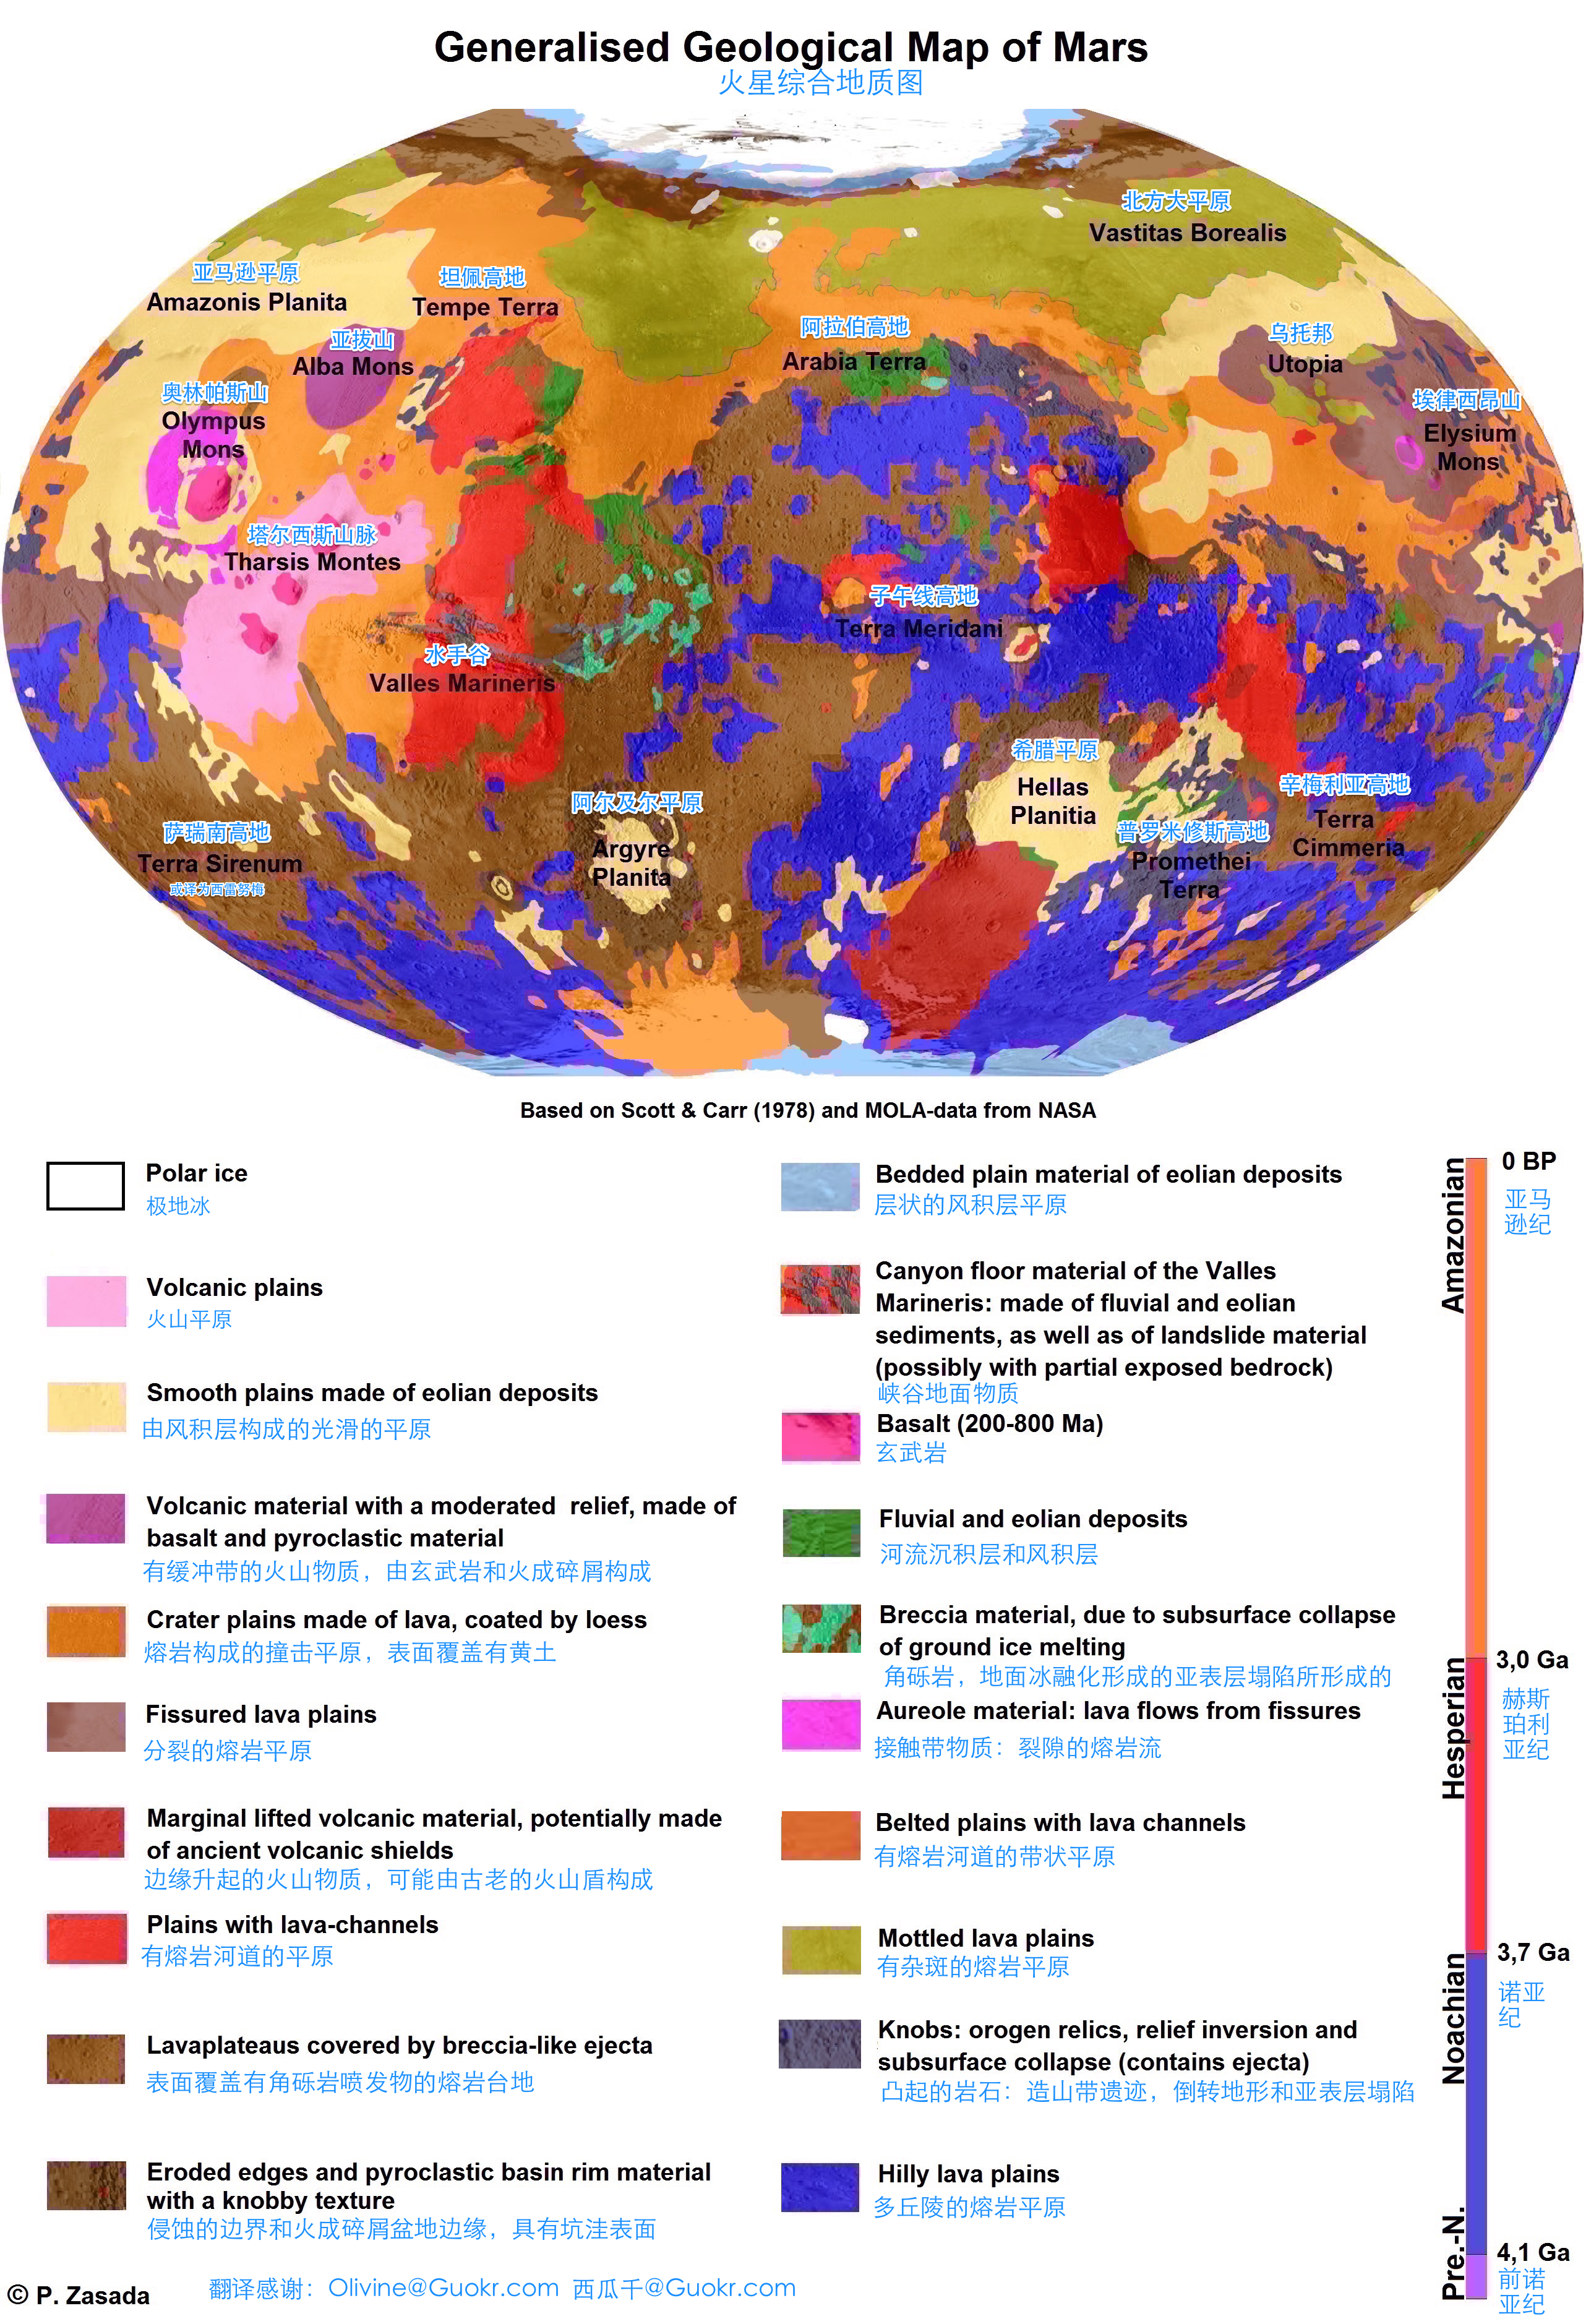
\includegraphics{GeneralisedGeologicalMapofMars.png}
\caption{翻译自 \href{https://commons.wikimedia.org/wiki/File:Generalised\_Geological\_Map\_of\_Mars.jpg}{Wikipedia} 。按照原图片的要求,翻译之后图片使用 \href{https://creativecommons.org/licenses/by-sa/3.0/deed.en}{Creative Commons Attribution-Share Alike 3.0 Unported} 协议共享。原作者为 Patrick Zasada 。}\end{figure}


\subsubsection{陨石坑}
\label{mars:id11}
火星上的陨石坑的命名规则是,大陨石坑以重要的科学家和科幻作家命名;小陨石坑则以地球上的村镇命名。一些主要的地形以及火星探测器标示在了下图中(红线为海平面分界线)
\begin{figure}[htbp]
\centering

\includegraphics{Mars24_1.png}
\end{figure}


\subsection{火星气候与天气}
\label{mars:id12}
在进行行星生态改造前,火星的天气一直不是特别好,沙尘暴特别严重。

火星轨道的偏心率是 0.09,要比地球轨道的偏心率的 0.02 大得多。这导致火星的气候的更加复杂。


\subsubsection{火星沙尘暴}
\label{mars:id13}\begin{figure}[htbp]
\centering
\capstart

\includegraphics{duststorms.jpg}
\caption{图片来自 \href{http://www.universetoday.com/14892/mars-dust-storms}{Universe Today} 。可以明显看到 2001 年 7 月 31 号的时候,整个星球都被沙尘暴覆盖了。}\end{figure}
\begin{figure}[htbp]
\centering
\end{figure}


\subsubsection{火星天气预报}
\label{mars:id15}
在移民火星之前,NASA 就开始对火星进行天气预报了:\href{http://www.msss.com/msss\_images/subject/weather\_reports.html}{Mars Weather Reports} 。


\subsubsection{火星气压}
\label{mars:id16}
火星的原来的气压也比较低,基本上在 1000Pa 左右,不适合人类居住。
\begin{figure}[htbp]
\centering
\end{figure}

\begin{notice}{note}{扩展阅读}
\begin{itemize}
\item {} 
\href{http://www.lpi.usra.edu/meetings/lpsc2010/pdf/1199.pdf}{Hargitai Henrik (2009). ``Climate Zones of Mars''. Lunar and Planetary Institute. Retrieved 2010-05-18.}

\end{itemize}
\end{notice}


\subsection{火星历法}
\label{mars:id18}
为了火星上的生活方便,火星上的计时与历法都与地球有所不同。

\index{火星计时}

\subsubsection{火星计时}
\label{mars:id19}\label{mars:index-0}
火星沿用了地球上秒、分钟以及小时,但是由于火星上一个太阳日的时间要比地球上的太阳日要长,因此火星上一天除了二十四个小时,还有一段的扩展时间,长度为 39 分 35.24409 秒。

文字记录方法在每天的二十四小时内与地球的记录方法相同,超出二十四小时的部分采用“+时间”来记录,例如二十四小时后十三分钟二十六秒记作:+13:26.

\index{火星历法}

\subsubsection{火星历法}
\label{mars:id20}\label{mars:index-1}
火星历法采用了大流士火星历,只是由于火星本地人的习惯的不同,对历法中的月份有不同的称呼,比较流行的是每年二十四个月分别采用了地球上古中国的二十四节气的称呼。火星历中,每个火星回归年定为一火星年,每年起始点为春分,是太阳直射火星赤道的时间。而火星元年开始,对应的是地球上的公元一九七零年四月二十八日,因此,人类第一个降落在火星的探测器,就是在火星元年到达的。

\index{火星月份}
火星历将每年分为二十四个火星月,按照每六个火星月一组分为四组,每组的前五个月有二十八个火星日,第六个月只有二十七个火星日,每年最后一个月在闰年会多包含闰日,即在闰年会有二十八天。一个典型的火星年应该是这样的。


\begin{threeparttable}
\capstart\caption{火星月份划分}

\begin{tabulary}{\linewidth}{|L|L|L|L|}
\hline

春季
 & 
夏季
 & 
秋季
 & 
冬季
\\

立春月(二十二月)
 & 
立夏月(四月)
 & 
立秋月(十月)
 & 
立冬月(十六月)
\\

雨水月(二十三月)
 & 
小满月(五月)
 & 
处暑月(十一月)
 & 
小雪月(十七月)
\\

惊蛰月(二十四月)
 & 
芒种月(六月)
 & 
白露月(十二月)
 & 
大雪月(十八月)
\\

春分月(一月)
 & 
夏至月(七月)
 & 
秋分月(十三月)
 & 
冬至月(十九月)
\\

清明月(二月)
 & 
小暑月(八月)
 & 
寒露月(十四月)
 & 
小寒月(二十月)
\\

谷雨月(三月)
 & 
大暑月(九月)
 & 
霜降月(十五月)
 & 
大寒月(二十一月)
\\
\hline\end{tabulary}

\end{threeparttable}


如表格所示,按照每六个月一个季节,分为四季。

\index{火星星期划分}
每个火星月共有四个星期,与地球不同的是,不管之前一个火星月最后一天是星期几,当每个火星月新开始的时候,星期总是从第一天开始计算。因此一个典型的火星月是这样的:


\begin{threeparttable}
\capstart\caption{火星星期划分}

\begin{tabulary}{\linewidth}{|L|L|L|L|L|L|L|}
\hline
\textsf{\relax 
星期日
} & \textsf{\relax 
星期一
} & \textsf{\relax 
星期二
} & \textsf{\relax 
星期三
} & \textsf{\relax 
星期四
} & \textsf{\relax 
星期五
} & \textsf{\relax 
星期六
}\\
\hline
1
 & 
2
 & 
3
 & 
4
 & 
5
 & 
6
 & 
7
\\

8
 & 
9
 & 
10
 & 
11
 & 
12
 & 
13
 & 
14
\\

15
 & 
16
 & 
17
 & 
18
 & 
19
 & 
20
 & 
21
\\

22
 & 
23
 & 
24
 & 
25
 & 
26
 & 
27
 & 
28
\\
\hline\end{tabulary}

\end{threeparttable}


最后一天是否存在与月份以及是否闰年有关。

火星年的置闰问题,算法与地球类似,即大流士火星历的置闰方法:
\begin{quote}

一火星日比一地球日长 39 分钟 35.244 秒,而一火星年的长度则为 668.5907 火星日,因此基本的置闰公式就是每十个火星年均由 6 个 669 火星日的火星年及 4 个 668 火星日的火星年所组成。前者(虽然比平年更常出现,可是仍然是被称作闰年)为奇数年份及能被 10 整除的年份。惟能被 100 整除的年份规定为平年;能被 1000 整除的年份为闰年;能被 3000 整除的年份为平年。
\end{quote}


\subsubsection{一些重要的日期}
\label{mars:id21}
作为历法的校准,火星元年一年中四个重要的日期与地球历法的对应为:


\begin{threeparttable}
\capstart\caption{火星元年月份}

\begin{tabulary}{\linewidth}{|L|L|L|L|}
\hline
\textsf{\relax 
春分
} & \textsf{\relax 
夏至
} & \textsf{\relax 
秋分
} & \textsf{\relax 
冬至
}\\
\hline
1970年4月28日
 & 
1970年11月12日
 & 
1971年5月15日
 & 
1971年10月8日
\\
\hline\end{tabulary}

\end{threeparttable}


火星上一些具有重要天文意义的节日:


\begin{threeparttable}
\capstart\caption{火星重要节日}

\begin{tabulary}{\linewidth}{|L|L|}
\hline
\textsf{\relax 
火星历日期
} & \textsf{\relax 
节日
}\\
\hline
春分月1日
 & 
火星春分
\\

芒种月12日
 & 
火星远日点
\\

夏至月27日
 & 
火星夏至
\\

寒露月11日
 & 
火星秋分
\\

大雪月12日
 & 
火星近地点
\\

冬至月14日
 & 
火星冬至
\\
\hline\end{tabulary}

\end{threeparttable}


\index{火星时区}

\subsubsection{火星时区}
\label{mars:index-4}\label{mars:id22}
由于火星上一天的时间并不是 24 小时,这给时期的划分造成了一定的麻烦。

为了时间换算的方便,火星上相邻两个时区之间时差均为 1 个小时,这样的话,一个时区的所跨的精度就不再是 15°,而是 14.5987°。

火星上的本初子午线为穿过艾里-0 陨石坑的经线,并且火星上的经度均以东经表示,从东经 0°-东经 360°,并没有西经,因此,火星上的时区也是以本初子午线为起点,向东每隔 14.5987° 为一个时区。这样一来,火星上最先进入一天的时区为 24 区,即靠近 0 区左侧的时区。火星上时区划分列表如下:


\begin{threeparttable}
\capstart\caption{火星重要节日}

\begin{tabulary}{\linewidth}{|L|L|L|L|}
\hline
\textsf{\relax 
时区
} & \textsf{\relax 
起始经度
} & \textsf{\relax 
终止经度
} & \textsf{\relax 
与0区时差
}\\
\hline
0区
 & 
0°
 & 
14.5987°
 & 
0
\\

1区
 & 
14.5987°
 & 
29.1974°
 & 
+1
\\

2区
 & 
29.1974°
 & 
43.7961°
 & 
+2
\\

3区
 & 
43.7961°
 & 
58.3948°
 & 
+3
\\

4区
 & 
58.3948°
 & 
72.9935°
 & 
+4
\\

5区
 & 
72.9935°
 & 
87.5922°
 & 
+5
\\

6区
 & 
87.5922°
 & 
102.1909°
 & 
+6
\\

7区
 & 
102.1909°
 & 
116.7896°
 & 
+7
\\

8区
 & 
116.7896°
 & 
131.3883°
 & 
+8
\\

9区
 & 
131.3883°
 & 
145.9870°
 & 
+9
\\

10区
 & 
145.9870°
 & 
160.5858°
 & 
+10
\\

11区
 & 
160.5858°
 & 
175.1845°
 & 
+11
\\

12区
 & 
175.1845°
 & 
189.7832°
 & 
+12
\\

13区
 & 
189.7832°
 & 
204.3819°
 & 
+13
\\

14区
 & 
204.3819°
 & 
218.9806°
 & 
+14
\\

15区
 & 
218.9806°
 & 
233.5793°
 & 
+15
\\

16区
 & 
233.5793°
 & 
248.1780°
 & 
+16
\\

17区
 & 
248.1780°
 & 
262.7767°
 & 
+17
\\

18区
 & 
262.7767°
 & 
277.3754°
 & 
+18
\\

19区
 & 
277.3754°
 & 
291.9741°
 & 
+19
\\

20区
 & 
291.9741°
 & 
306.5728°
 & 
+20
\\

21区
 & 
306.5728°
 & 
321.1715°
 & 
+21
\\

22区
 & 
321.1715°
 & 
335.7702°
 & 
+22
\\

23区
 & 
335.7702°
 & 
350.3689°
 & 
+23
\\

24区
 & 
350.3689°
 & 
360°
 & 
+24
\\
\hline\end{tabulary}

\end{threeparttable}


必须注意的是,24 区所横跨的经度并不是 14.5987°,而是 9.6311°。第二十四时区为附加时区,即为负责调整火星上比 24 小时多出来的 39 分 35.24409 秒的时区。


\section{星际移民历史}
\label{history::doc}\label{history:id1}
星际移民有着一段悠久的历史。血与泪,悲与喜,星际移民并非一蹴而就。


\subsection{2027 首次载人登火}
\label{history:id2}

\subsubsection{世纪发现}
\label{history:id3}
2020 年以前,人类对于火星的探索都还局限于使用探测器和火星车的无人探测。2021 年,载人登火计划启动,人类向着红色行星迈出了真正意义上的“第一步”。这一切,都还要得益于 \href{http://en.wikipedia.org/wiki/ExoMars}{ExoMars} 从火星传回的喜讯。

ExoMars 任务是由欧空局(ESA)与俄罗斯联邦航天局(Roscosmos)合作进行的火星探索任务,它的主要目标在于寻找可能存在的火星生命。2019 年,ExoMars 在火星表面的 \href{http://en.wikipedia.org/wiki/Mawrth\_Vallis}{马沃斯谷} 附近着陆,开始巡视探索。和好奇号火星车一样,ExoMars 也能采集火星表面的岩石样品,并对其中可能存在的有机物分子进行分析。
\begin{figure}[htbp]
\centering
\end{figure}

经过了两年多的火星探索,2020 年 3 月,欧空局和俄罗斯联邦航天局联合对外宣布,ExoMars 发现了“火星上有机物存在的关键性证据”,“红色星球存在过远古生命的可能性大大增加”。消息一传出,立刻轰动了整个世界,人类对火星的探索热情异常高涨。

\index{赤风计划}
\index{Red Storm}

\subsubsection{“赤风(Red Storm)”计划启动}
\label{history:red-storm}\label{history:index-1}
2021 年 1 月 1 日,美国、俄罗斯、欧空局 20 国、加拿大、中国、日本、印度、以色列 27 个国家共同宣布,人类的首个载人登火计划启动,代号“赤风”。人类将在 2027 年登陆火星!如此大规模的航天国际合作史无前例,各国航天局的协调工作由 \href{http://en.wikipedia.org/wiki/United\_Nations\_Committee\_on\_the\_Peaceful\_Uses\_of\_Outer\_Space}{联合国和平利用外层空间委员会(简称COPUOS)} 统一完成。

载人登火任务耗资巨大,如果只由一个国家完成可能会拖累其经济,因此,以国际合作的形式启动载人登火计划,确实能分摊成本,减小风险。在各国经过反复的磋商之后最终决定,采用最保守的方案将人类送往火星:
\begin{itemize}
\item {} 
先利用重型运载火箭进行发射,将飞船的各个部件送往近地轨道;

\item {} 
接着在近地轨道上完成飞船的组装;然后从近地轨道出发,前往火星;

\item {} 
进入绕火轨道后,载有宇航员的着陆舱与飞船分离,准备软着陆火星表面;

\item {} 
着陆之后,宇航员将在火星上开展接近一年的探索、实验活动;

\item {} 
火星探索结束后,宇航员乘坐上升器返回停泊在绕火轨道上的飞船;

\item {} 
飞船从火星轨道出发,开始返回地球;

\item {} 
接近地球后,宇航员进入另一个着陆舱返回地球表面,任务结束。

\end{itemize}

在确定了载人登火方案之后,各国紧锣密鼓地开展了具体的研究和制造工作。经过 \href{http://en.wikipedia.org/wiki/Space\_Launch\_System}{SLS火箭} 的 6 次发射,一个重量近 500 吨,使用氢氧燃料作为推进剂的飞船在近地轨道上组装完成。

2027 年 1 月 6 日,装载着 4 名宇航员和生活舱的最后一枚 SLS 火箭发射升空,与近地轨道上的飞船完成对接。在完成最后的调试工作后,飞船点火离开了蓝色星球,向着远方的红色星球飞去。
\begin{figure}[htbp]
\centering
\end{figure}


\subsubsection{人类登陆火星}
\label{history:id5}
一切活动都按着当初的计划有序开展。2027 年 7 月 22 日,经过多次变轨,飞船最终进入 500km 绕火轨道。不久,3 名宇航员进入着陆舱,并与飞船分离,剩下一名宇航员留在飞船内部工作。

7 月 23 日,着陆舱突破火星的大气层,最终降落在火星乌托邦平原边缘的阿蒙蒂斯区(23.27°N 109.08°E),这一天,人类的脚印终于印在了这颗红色星球之上!
\begin{figure}[htbp]
\centering

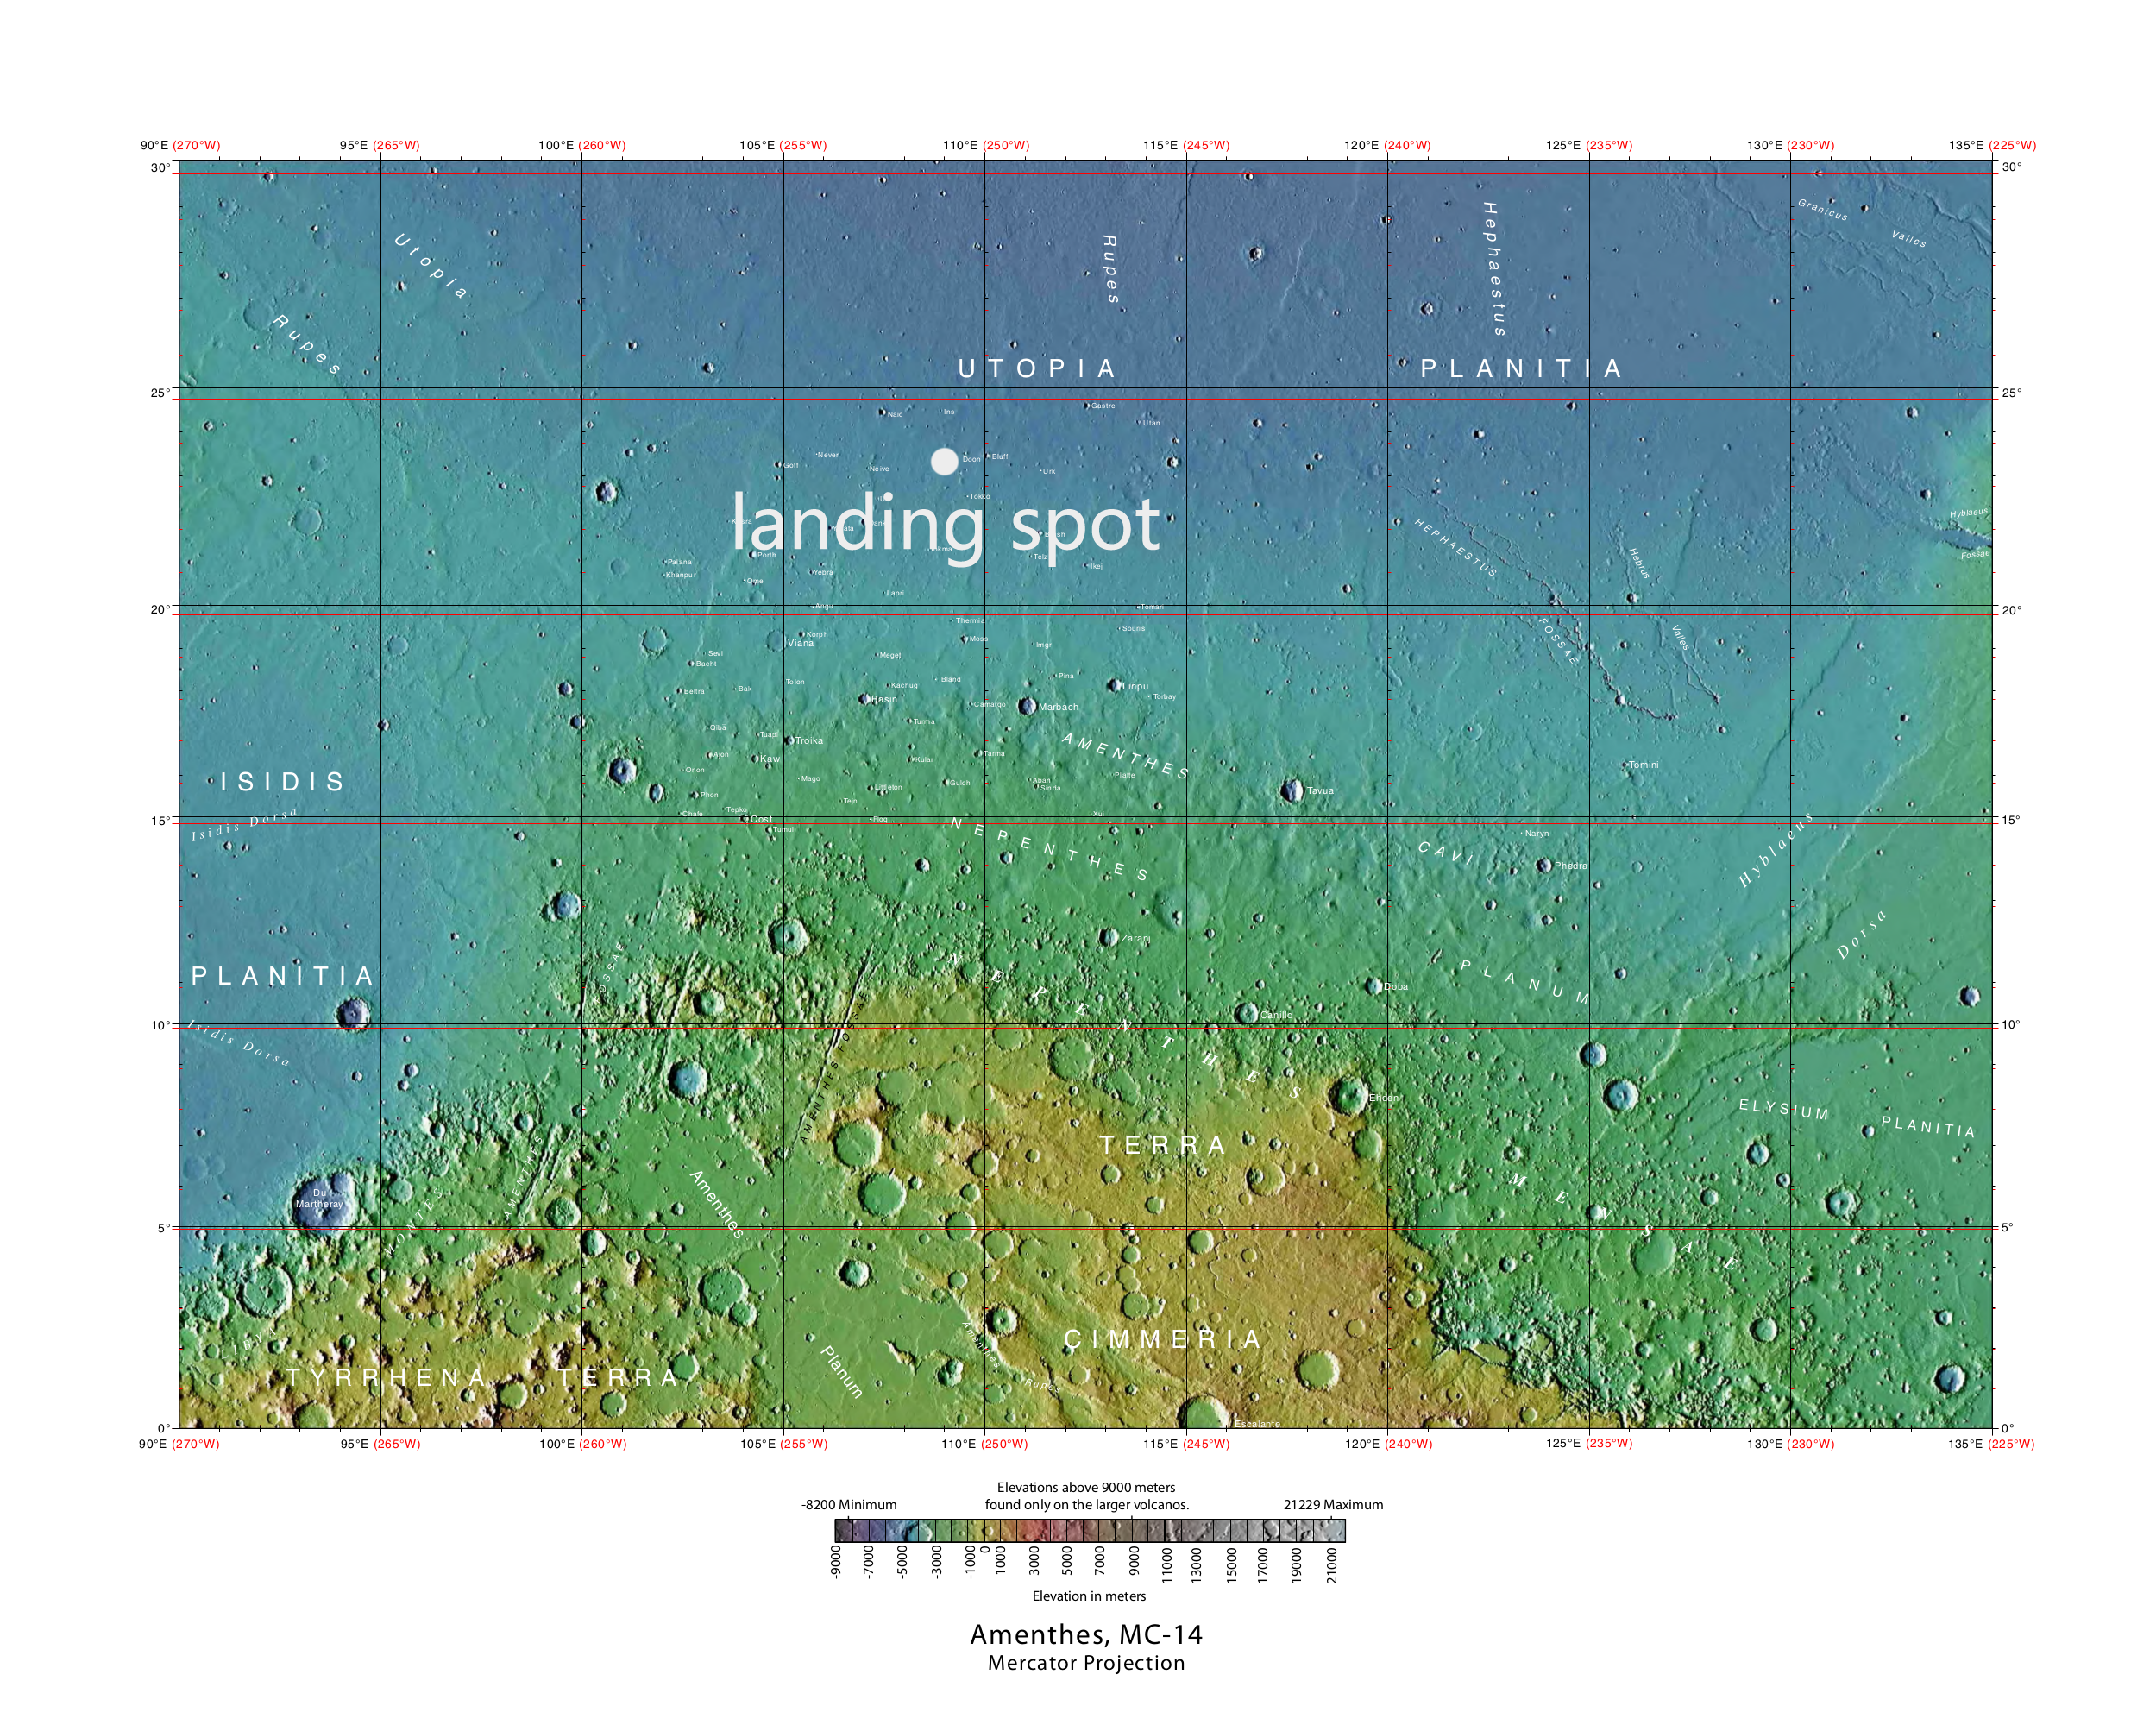
\includegraphics{landing_spot.png}
\end{figure}

在为期 300 余天的火星探索活动中的大多数时间里,宇航员是在生命保障舱内度过的。他们在舱内完成了众多实验,包括测试了植物、微生物在火星环境下的生长情况,火星大气中二氧化碳转化成氧气的实验,火星土壤中的金属冶炼实验等等。由于宇航服储氧量的限制,舱外活动时,宇航员只能前往离着陆点较近的地方,一般的舱外活动时间在六小时左右,宇航员将选择并采集火星表面的岩石样品,并将其带回地球供科学家分析。

2028 年 5 月 19 日,在完成所有预定任务后,宇航员乘坐上升器离开火星表面,与停泊在绕火轨道上的飞船进行对接。航天员进入飞船后,抛掉上升器,飞船再次点火飞向地球。2029 年 2 月 8 日,载有宇航员的着陆舱成功降落在地球表面,“赤风”载人登火计划取得成功。


\subsection{2030-2060 小行星开发热潮}
\label{history:id6}

\subsubsection{国际合作的破裂}
\label{history:id7}
“赤风”计划的成功,让地球上的人们看到了火星探索的新希望,当时很多人认为,火星探索的热潮就此开始,接下来的载人登火任务也会在几年内启动。可是,国际政治形式的风云变幻让这一切都化为泡影。参与载人登火任务的各国对于火星采集样品的分配、载人登火技术分享等等问题上产生了严重的分歧,名义上统筹整个计划的 COPUOS 在载人登火成功之后没了权力,要想再开展第二次载人登火任务已近乎不可能,人类史上最大规模的一次国际合作逐渐走向破裂。

\index{太空产业化}
\index{Space Industrialization}

\subsubsection{太空产业化(Space Industrialization)}
\label{history:space-industrialization}\label{history:index-3}
第一次载人登火之后的 30 年,只有少数几个国家再向火星发射过无人探测器,航天大国纷纷将发展的重点放在了“太空产业化”的方向上。由于航天领域的进入门槛较高,前期投资巨大,没有国家的扶持,初期建立起的公司很难有竞争力。因此,各国纷纷扶持本国的建立起的航天公司,希望能将外太空开发成为促进本国经济增长的热土。

在太空产业化的过程中,有不少产业逐渐发展起来,这其中包括了:

\index{太空运输业}
\index{Space Transportation Industry}\begin{itemize}
\item {} 
\textbf{太空运输业(Space Transportation Industry)}:从早期的太空发射业发展起来,逐步发展为天地运输(地球\(\rightarrow\)低轨道)、地球轨道运输(低轨道\(\rightarrow\)高轨道、地球轨道\(\rightarrow\)月球)、行星际运输(地球轨道\(\rightarrow\)小行星/火星)等;

\end{itemize}

\index{太空通信业}
\index{Space Communication Industry}\begin{itemize}
\item {} 
\textbf{太空通信业(Space Communication Industry)}:从早期的卫星产业发展起来,逐步发展为地球通信(地球\(\rightarrow\)卫星\(\rightarrow\)地球)、地月通信(地球\(\rightarrow\)卫星\(\rightarrow\)月球)、行星际通信(地球\(\rightarrow\)卫星\(\rightarrow\)小行星/火星)等;
\begin{figure}[htbp]
\centering

\includegraphics{DSI-Firefly-concept_BV-21-01-13.jpg}
\end{figure}

\end{itemize}

\index{太空旅游业}
\index{Space Tourist Industry}\begin{itemize}
\item {} 
\textbf{太空旅游业(Space Tourist Industry)}:从早期的亚轨道旅游发展起来,逐步发展为亚轨道旅游、轨道旅游、月球旅游等;

\end{itemize}

\index{太空能源业}
\index{Space Energy Industry}\begin{itemize}
\item {} 
\textbf{太空能源业(Space Energy Industry)}:21 世纪 20 年代发展起来的新兴产业,早期主要为在轨卫星、探测器提供燃料补给,后来扩展到小行星燃料生产;
\begin{figure}[htbp]
\centering

\includegraphics{DSI-FuelProcessor_BV-20-01-13.jpg}
\end{figure}

\end{itemize}

\index{太空采矿业}
\index{Space Mining Industry}\begin{itemize}
\item {} 
\textbf{太空采矿业(Space Mining Industry)}:和太空能源业同时建立起来的新兴产业,以小行星开发为基础,主要包括矿石的开采、冶炼,涵盖了铁、镍、钴、铂族金属、半导体元素等等;
\begin{figure}[htbp]
\centering

\includegraphics{DSI-settlement-concept_BV-21-01-13.jpg}
\end{figure}

\end{itemize}

\index{太空制造业}
\index{Space Manufacturing Industry}\begin{itemize}
\item {} 
\textbf{太空制造业(Space Manufacturing Industry)}:以太空能源业和太空采矿业为基础,主要进行微重力条件下的产品制造。小行星表面、地球轨道、月球表面均建有太空工厂,生产的产品大多用于太空中基础设施的建立,少量产品将被运回地球。
\begin{figure}[htbp]
\centering

\includegraphics{future-asteroid-mining-2030s.jpg}
\end{figure}

\end{itemize}

\index{太空商业联合会}
\index{Space Business Federation}

\subsubsection{太空商业联合会的建成}
\label{history:index-17}\label{history:id8}
在太空产业化浪潮的影响下,众多的航天公司、太空企业如雨后春笋般地发展起来。不管是 LEO、GEO、月球轨道、小行星轨道,还是月球表面、小行星表面,都有着巨大的商业开发价值。由于太空产业其特有的利润巨大、投入巨大、风险极高的性质,相同领域的太空企业纷纷组成各自的商会,分摊成本、共同开发潜力巨大的太空市场。主要的太空商会包括了:

\index{联合发射同盟}
\index{United Launch Alliance}
\index{ULA}\begin{itemize}
\item {} 
\textbf{联合发射同盟(United Launch Alliance,简称 ULA)}:最初是 2006 年由洛克希德马丁公司和波音公司创立的合资企业,太空产业化浪潮到来之际,又有一些新成立的太空运输业公司加入了 \href{http://en.wikipedia.org/wiki/United\_Launch\_Alliance}{ULA} ,主要业务集中在天地运输、地球轨道运输。
\begin{figure}[htbp]
\centering
\end{figure}

\end{itemize}

\index{宇宙通信卫星组织}
\index{Universal Telecommunications Satellite Organization}
\index{Unisat}\begin{itemize}
\item {} 
\textbf{宇宙通信卫星组织(Universal Telecommunications Satellite Organization,简称 Unisat)}:由国际通信卫星组织( \href{http://en.wikipedia.org/wiki/Intelsat}{Intelsat} )、国际海事卫星组织( \href{http://en.wikipedia.org/wiki/Inmarsat}{Inmarsat} )、欧洲通信卫星组织( \href{http://en.wikipedia.org/wiki/Eutelsat}{Eutelsat} )、亚洲卫星公司( \href{http://en.wikipedia.org/wiki/AsiaSat}{AsiaSat} )逐渐合并而成,业务囊括了整个太空通信业,并且几乎垄断了地球通信市场。

\end{itemize}

\index{联合小行星}
\index{United Asteroid Institution}
\index{UAI}\begin{itemize}
\item {} 
\textbf{联合小行星(United Asteroid Institution,简称 UAI)}:由行星资源公司( \href{http://www.planetaryresources.com}{Planetary Resourses} )、SpaceX小行星公司(SpaceX Asteroid)、深空工业公司( \href{http://deepspaceindustries.com}{Deep Space Industry} )、近地小行星矿业公司(NEAs Mining)组合而成,后来又合并了一些新成立的太空采矿公司,基本垄断了小行星采矿、小行星燃料生产、小行星产品制造市场。

\end{itemize}

\index{轨道旅游局}
\index{Orbital Travel Agency}
\index{OrbiTA}\begin{itemize}
\item {} 
\textbf{轨道旅游局(Orbital Travel Agency,简称 OrbiTA)}:由维珍银河公司( \href{http://en.wikipedia.org/wiki/Virgin\_Galactic}{Virgin Galactic} )、宇宙探险公司(宇宙探険株式会社)、SpaceX旅游(SpaceX Tourist)合并而成,主要开发亚轨道、近地轨道旅游、近地空间站旅游等等。

\end{itemize}


\subsubsection{载人火星探索的冷落}
\label{history:id9}
21 世纪 30 年代到 60 年代,是一个公司主导太空开发的时代。第一次载人登火计划虽然成功,但是国际合作破裂之后,耗资千亿美元的旅程却让任何一个国家都无法轻松承担。相比近地小行星开发,火星开发的短期价值极低,火星上的并没有地球上稀缺的矿产,去一趟火星消耗的燃料也比去小行星要多得多。因此,这 30 年来,红色星球一直无人问津,偶尔有承担科研任务的机器人孤零零地降落在火星表面,一直工作到停转的最后一刻。

\index{火星轨道游}
唯一和火星近距离接触的机会是轨道旅游局开发的“火星轨道游”线路,飞船从地球出发,历经 200 余天到达火星轨道,从太空俯瞰它的美景之后,又历经 200 余天返回地球。这条旅游线路的价格极贵,一般的富豪都难以承担。而且旅游的时间跨度接近两年,其中只有 5\% 的时间停泊在火星轨道,其余的时间均在太空中航行。如此长时间地在太空中生活,一般人也是消受不起的。最终,也只有一对来自美国的夫妇订购了此条线路,他们也成为了这几十年来最为靠近火星的人。


\subsection{2060-2070 星际移民局成立}
\label{history:id10}

\subsubsection{太空产业化的后续影响}
\label{history:id11}
持续了近 30 年的太空产业化浪潮,在很大程度上改变这个世界的面貌。相同领域的太空企业组成的太空商会,不仅在经济上把控着人类社会的命脉,更影响着整个世界的政治格局。太空商会慢慢地从一个个富可敌国的经济实体转变为真正有影响力的政治实体,不过在国际法律上,太空商会的政治地位还没有得到传统国家的广泛认同,但大部分的人认为,这种“认同”也只是时间问题罢了。除此之外,太空产业化给人类社会带来的影响还包括了:


\paragraph{航天技术的飞速发展}
\label{history:id12}
在 21 世纪上半叶,航天对于大多数人来说还只是高技术、高投入、高风险的代名词。火箭发射的成本高居不下,新型的火箭引擎迟迟无法在实际中派上用场,这一切,都让人们觉得太空离我们是那么得遥远。不过,20 世纪 20 年代,随着航天市场的逐渐开放,一些私营企业逐步参与到发射市场的竞争中来,它们为了最大限度降低成本而开发的“可重复使用技术”可以说迈向了航天“低成本化”、“可重复化”的第一步,也为整个“太空产业化”拉开了序幕。

在这之后,航天成本逐步减低,太空市场的竞争日趋强烈,要想在这之中占有一席之地,除了与组建的太空商会一起抱团取暖之外,不断研发出领先的航天技术才能保证自己不被淘汰。在此意义之下,航天技术的飞速发展不仅给太空企业带来了活力,更加快了整个人类社会迈向太空的步伐。这些新的航天技术包括了:
\begin{itemize}
\item {} 
\textbf{太空燃料补给技术}

\item {} 
\textbf{太空激光通信技术}

\item {} 
\textbf{太空3D打印技术}

\item {} 
\textbf{封闭环境生态循环技术}

\item {} 
\textbf{微重力环境制造技术}

\item {} 
\textbf{近地轨道电磁投射技术}

\item {} 
\textbf{大推力离子引擎技术}

\item {} 
\textbf{小行星采矿技术}

\item {} 
\textbf{小行星氢氧燃料生产技术}

\end{itemize}


\paragraph{近地太空市场(Near-Earth Space Market)开发殆尽}
\label{history:near-earth-space-market}
所谓近地太空,并不是指近地轨道(Low Earth Orbit)的太空。狭义的近地太空指的是地球影响球以内的空间,包括了近地轨道、地球同步轨道以及月球在内的空间;广义的近地太空还囊括了近地小行星、地日拉格朗日 L1、L2、L4、L5 点附近的空间。虽然近地太空中的资源数不胜数,但是真正有商业开发价值的还是很少。
\begin{figure}[htbp]
\centering
\end{figure}

首先说月球,虽然月球表面有丰富的氦-3 资源,但是由于氦-3 均匀分布在表层的月壤之中,开采、提取难度很大,况且人类尚未掌握成熟的核聚变技术,因此月球的氦-3 资源暂且是可望而不可即。

再来说近地小行星,现已开发成熟的 \href{http://en.wikipedia.org/wiki/Near-Earth\_object\#Near-Earth\_asteroids}{近地小行星} 主要是含水较丰富的 C 型小行星以及含金属较丰富的 M 型小行星,但并不是所有的 C 型、S 型小行星都有开发价值。由于近地小行星绕太阳运行的轨道与地球轨道相近,这也就注定了其与地球的汇合周期较长,也就是说,对于一颗特定的小行星,需要等较长的时间才能迎来一次发射窗口或者返回窗口,这给太空采矿增加了不小的难度。

考虑到这些因素,近地太空市场可供开发的空间还是很有限的。截至 21 世纪 50 年代末期,在当时技术下有利可图的 200 余颗小行星几乎都已经“名花有主”了。
\begin{figure}[htbp]
\centering
\end{figure}

\index{泛火星思潮}

\paragraph{“泛火星思潮”的蔓延}
\label{history:index-31}\label{history:id14}
就像“阿波罗计划”成功后的50多年里月球再也无人踏足一样,“赤风计划”成功后的 30 多年里,火星也一直无人问津,历史以它惊人的相似性给地球人开了一个莫大的玩笑。对于太空产业化,地球人普遍采取了两种互相对立的观点。一种观点认为,太空产业化促使航天技术迅猛发展,同时也让全世界的人类都感受到了太空带来的福祉,人类正在一步一步迈向广阔的太空;另一种观点认为,太空产业化催生了一个又一个富可敌国、左右政局的太空商会,太空商会垄断着太空中的方方面面,却始终将开发的范围局限在近地太空,深空探索一点一点地被冷落,火星移民更是无从谈起,太空产业化实质上阻碍了人类迈向太空的进程。

初期时,两种观点互不相让,而在产业化后期,第二种观点则被更多的地球人所认同,并称之为“泛火星思潮”,这种思潮呼吁打破太空商会对于太空商业开发的垄断,并呼吁人类应该尽早开始火星移民。
\begin{figure}[htbp]
\centering
\end{figure}

\index{联合行星}
\index{United Planet Institution}
\index{UPI}

\subsubsection{联合行星(United Planet Institution)的成立}
\label{history:united-planet-institution}\label{history:index-34}
近地太空市场开发殆尽再加上“泛火星思潮”的蔓延,使得太空商会不得不把目光投向红色星球,否则,商会的资金来源、声望地位都会受到不利的影响。2060 年,UAI(联合小行星)公布了未来的发展蓝图,宣布将把商会的开发领域拓展到火星,在火星上建成首个人类殖民地,并发展相关的火星产业。同年,UAI宣布更名为 UPI(United Planet Institution,联合行星),并声称火星移民计划已进入准备阶段。
即使是已经坐拥 100 余颗小行星的 UPI,在火星移民的问题上,也不敢莽撞行事。由于太空商会在地球上的声誉普遍较差,即使UPI利用自身政治影响力,通过一些“隐藏手段”获得了几个联合国常任理事国的支持,UPI 也不易让普通民众相信其所描绘的“火星移民蓝图”,因而一度陷入了信任危机。

\index{星际移民局}
\index{Interplanetary Immigration Agency}
\index{IIA}

\subsubsection{星际移民局(Interplanetary Immigration Agency)的成立}
\label{history:interplanetary-immigration-agency}\label{history:index-37}
2062 年 7 月 23 日,在登火 35 周年的纪念日这一天,联合国宣布人类历史上第一家正式从事星际移民的机构————IIA (星际移民局)成立了。
\begin{figure}[htbp]
\centering

\includegraphics{InterImm_banner_white_1720X430.png}
\end{figure}

在形式上,IIA 属于联合国的下属机构,负责统筹人类的星际移民工作(在眼下当然主要负责火星移民),这包括招募、选拔、培训火星移民志愿者,开展火星移民相关技术的研究,在初期移民过程中提供资金、技术、工具、补给,甚至还包括了火星生态改造的研究。根据联合国的声明,IIA 的主要资金来源于成员国划拨的预算,少量资金来源于太空商会,但实际上,IIA 的资金援助、技术支持几乎全由 UPI 提供,只不过通过联合国这块牌子,赢取地球人的信任感罢了。在很多地球民众的眼里,IIA 甚至还成了与 UPI 对抗的一个高大形象存在,这让地球人对 IIA 的好感度倍增,自然对其所提出的火星移民计划信心十足。


\subsubsection{火星移民计划启动}
\label{history:id15}
IIA 成立之后,火星移民计划顺势启动。按照 IIA 提出的构想,第一阶段的火星移民将分为三步来实现:利用 50 年的时间,在火星上建成第一个人类殖民地。按殖民地的规模,其建设阶段将分为火星前哨站(Mars Outpost) \(\rightarrow\) 火星基地(Mars Base) \(\rightarrow\) 火星城市(Mars City)。在第一阶段完成之前,不考虑进行其他殖民地的建设以及火星生态改造。


\paragraph{首批火星移民志愿者选拔}
\label{history:id16}
移民计划启动之后,IIA 发布了首批火星移民志愿者的招募通知,吸引了全世界的关注。首批移民志愿者计划招募 60 人,将分为 4 队送往火星殖民地。招募的要求包括了:年龄 18-40 岁;身体强壮、心理素质良好;拥有一门以上的专业技能或知识;至少掌握一门外语。值得一提的是,在招募要求中 IIA 明确提出,移民志愿者在第一阶段开展的 50 年内不得返回地球、并且不得生育。据 IIA 的官员解释,不得返回地球是因为这样会在殖民地建设阶段耗费额外的资金,而不得生育则是考虑到了火星表面的辐射可能对胎儿和孕妇造成的不利影响。

虽然招募通知中有着一项项严苛的条件,但这却挡不住地球人争相报名的步伐,对红色星球的向往之情在蓝星上彻底点燃。在报名的人当中,大部分是 30 岁以下的年轻人,他们可能才踏入社会不久,在地球上尚未拥有一个美满的家庭,这样就省去了不少对于家庭的挂念,期待着能在火星上燃烧自己的青春。当然,IIA 也不会只挑选年轻人,整个移民团队中也需要经验丰富的人指引方向。因此,一些曾在太空中工作过的宇航员也会被选入移民志愿者的队伍。

经过一年多的选拔,来自世界各地的 60 名志愿者(36 名男性,24 名女性)被选拔出来。这其中 40 人年龄在 30 岁以下,12 人年龄在 30-35,剩下 8 人年龄小于40(报名登记时,也就是2062年时的年龄)。在经过长达 6 年的训练后,他们在 2069 年 8 月 5 日启程离开地球,前往火星。


\paragraph{殖民地建设前期准备}
\label{history:id17}
在火星移民志愿者招募进行的同时,IIA 也开展了殖民地建设的准备工作。在小行星采矿兴起的时期,UAI 就已经在 LEO 上建成了两个电磁投射器,电磁投射器使用太阳能进行充电,能够承担小行星轨道⇔近地轨道、近地轨道\(\rightarrow\)地面的投射/接收工作。电磁投射器还使用了大推力离子引擎进行自身的轨道维持。不过,电磁投射器并不能投射所有的东西,由于投射时的过载极大,它无法进行载人运输,只能用于货运。此外,货物也必须装在专门的动力投射舱中才能进行运输,这是由于改变航天器轨道的敏感度极高,想要把无动力的货物准确投射到预定地点几乎不可能,而动力投射舱上安装有离子引擎,能够在航行途中进行轨道修正,因此才能够承担货运任务。

IIA 首先将一个电磁投射器运送到火星轨道,用于接收地球投射过来的货物。另一方面,一些精密的舱段、仪器、机器人等则使用消耗氢氧燃料的货运飞船进行运输,这些飞船会在小行星燃料补给站进行燃料补充。

在火星移民正式出发前,登陆点附近就已经有不少从地球运送过来的货物和舱段,包括了生活舱段、核电舱段、种植舱段、医疗舱段、食物、水、火星车、机器人等等。


\subsubsection{火星移民登陆}
\label{history:id18}
2070 年 4 月 22 日,首批火星移民志愿者第 1 远征队的 15 人在伊希地平原的西北地区(16.181°N,84.624°E)着陆,人类新的篇章就此展开!
\begin{figure}[htbp]
\centering
\end{figure}


\subsection{2070-2100 火星殖民地建设}
\label{history:id19}
火星殖民地的建设并不是单纯的火星地面的发展,而是火星表面、绕火轨道、小行星产业和地球太空产业的共同进步,从某种意义上说,这是各大太空商业联合会合作的成果。在早期的建设中,小行星产业、太空运输业和火星的建设几乎完美地协调发展,特别是太空运输业的发展,使得火星殖民地的建设有了极强的后备保障。


\subsubsection{建设初期}
\label{history:id20}
2070 年 4 月,联合行星(UPI,前联合小行星,即 UAI)的首个火星表面前哨站在伊希地建立之后,基础设施并不完善,地面的生活基本上只能满足最低生活需求。这些先驱们在恶劣的环境中努力建设着殖民地,他们的壮举,成就了之后火星的繁荣。

次年,其他商业联合会包括联合发射同盟(ULA)、宇宙通信卫星组织(Unisat)以及新兴的推进技术发展组织(Promotion of New Propulsion Technology,简称PNPT)也迅速加入到火星殖民地的建设中来。到 2075 年,ULA、Unisat 和 PNPT 提供的围绕火星的大型飞船及空间设施曾经一度达到十二艘。这些空间设施有着各自的使命,从能源供给到太空运输,从机械维修到生命保障,他们组成了整个火星殖民地坚实的后备保障。随着火星殖民地逐渐完善,很多大型设施从轨道转移到了火星表面。

值得一提的是,Unisat 提供的包括气象卫星、定位系统和遥感卫星等在内的卫星系统为火星表面殖民地的建设提供了各种便利。

\index{地火运输}

\subsubsection{地火运输}
\label{history:index-38}\label{history:id21}
地球和火星之间的物资运输曾经一度成为整个火星开放计划中耗资最大的部分,这也曾经是 IIA 的研发部门投入精力最多的一个问题。2075 年,PNPT 正式并入 IIA,之后的 20 年内,太空运输业的发展达到巅峰时期。

在经历了短暂的传统化学火箭推进之后,热核火箭和离子推进迅速崛起,地球-火星航线变得更加快捷安全。

\begin{notice}{note}{地火运输}

关于地火运输的技术知识,请参阅 \href{http://interimm.org/InterImmBook/tech.html\#earth2mars-foldin}{科技-地火运输} 。
\end{notice}


\subsubsection{能源供给}
\label{history:id23}
由于太阳能电站可以迅速搭建起来,并且成本很低,火星殖民地建设的早期大量使用太阳能。第一个建立起来的是太空太阳能电站“太阳神一号”,除了为轨道上的飞船提供能源补充,也能无线传输给地面使用。第二个太阳能电站,也就是第一个地面电站,在地面殖民地安顿下来之后就开始施工并在短短几天内完成。

火星春秋季的沙尘暴严重影响太阳能电站的效率,IIA 决定建立风电站和核电站。到 2080 年为止,火星殖民地的能源供给就已经形成了以核电为核心,风能和太阳能辅助的能源体系。


\subsubsection{绕火轨道}
\label{history:id24}
在 2071 年之前,绕火轨道上只有 Unisat 提供的遥感卫星和通信卫星。为了配合太空运输系统和地面殖民地的建设,Unisat 增加了多颗火星卫星。此外,ULA 和 IIA 联合发射的火星空间站等配套设施也逐步建立起来。遥感卫星对于火星表面灾害性天气的预警预测,使得地面建设可以避开糟糕的天气情况。而空间站在建设时期主要起到了太空运输货物中转的作用。


\subsubsection{地面建设}
\label{history:id25}
火星殖民地的第一个地面加工厂是燃料工厂,该工厂在第一批火星开拓者到来之前就已经开始运行了。在前哨站建立以后,燃料工厂被扩建,2075 年已经能够基本满足火星表面与绕火轨道上之间运输的燃料需求。

利用 UPI 的小行星矿场运来的液氢,结合火星大气中的二氧化碳,燃料工厂可以生产甲烷、氧气以及醇类。液体燃料除了少部分给地面运输车辆作为燃料之外,大部分用于火星表面和轨道之间的运输。随着地面设施的完善,地面矿场开始投入使用,由于原料和能源的限制,矿业只是为火星殖民地的建设所服务。

配合大型电站、燃料工厂、空气工厂和水工厂,其他的后备生活设施也建立起来。大型温室建立之后,火星地面殖民地能够容纳的人员越来越多,建设步伐也极大地加快了,甚至很快建立起了运输、采矿、冶炼、化工和制造的工业链。主要的材料来源从初期的小行星矿场,转变为殖民地的工厂。很多机械的制造,包括建筑 3D 打印机,也实现了独立生产。

2080 年,轨道旅游局(OrbiTA)也开始大规模投资火星殖民地的旅游开发,并开始优化火星的天地运输系统。

原本只关注地球上的产业的一些重工业公司,也开始往火星投资。配合地球运输来的机器人核心模块,火星殖民地组装了多架工业机器人,从材料运输到更加大型的建筑 3D 打印,机器人大大加快了建设的步伐。


\subsubsection{科学探索}
\label{history:id26}
建设时期,火星的科学探索也欣欣向荣。建设初期的科学主要集中在考古,地质,农业,生态和物理,尤其是火星考古几乎成为大众关心的科学焦点。火星农业和生态学的发展,使得后来的大型生态圈工程成为可能。

绕火轨道上的空间站也逐步扩展为研究人员基地。由于很多推进器测试都选择了地球到火星的轨道,部分推进器研究机构都往火星空间站派驻了研究人员。UPI 的推进技术研究中心甚至在绕火轨道设立了单独的空间站,为其研究人员提供生活和研究的空间。

\index{星际通信公司}
\index{Interplanetary Communication Company}
Unisat 的重要成员 \textbf{星际通信公司(Interplanetary Communication Company)} 也在火星表面和绕火轨道设立研究中心。
\begin{figure}[htbp]
\centering
\end{figure}


\subsection{2100-2120 火星移民热潮}
\label{history:id27}
多个大型生态圈的建立,推进了第一个火星移民热潮。很多的商人巨贾在退休之后选择来到重力比地球小的火星来安享时光。有些年轻人认为建设时期的火星有很多成功的机会,也都争先移民到火星来创造自己的未来。另外由于火星提供了很多跟地球不同的环境,大量的不同研究方向的科研人员也选择长期居住在火星。火星独特的环境,重新点燃了很多发展缓慢的学科,衍生出了新的研究方向,学科交叉也变得更加显著。

\index{四大商会合并}
\index{星际移民中心}
2102 年 6 月,Unisat、ULA、OrbiTA 与 UPI 合并,保留 UPI 的名称。四大商会合并,一时间成为人人皆知的热门话题。借着合并的春风,火星殖民地的建设投入大大增加,吸引了大量的地球企业前来投资。尤为突出的是 \textbf{行星生态公司} 。这原本是一家地球的环保公司,但是投入了大量的科研经费,其中小型的生态循环的研究非常出色。该公司为火星殖民地开发了多种生态圈,公司股票一时间也是炙手可热。2113 年,该公司被 IIA 收编,但是保留了原来的公司形态。次年,IIA 将部分非盈利的部门拆分重组为 \textbf{星际移民中心} ,研发和服务部门大多成为星际移民中心的一部分。而剩余的部分大多由盈利的公司构成,逐渐成为星际移民中心的经济来源。火星移民热潮中,IIA 由原来的 UPI 提供经济支持,逐渐发展成为经济独立的机构。


\subsubsection{火星殖民地更加完善}
\label{history:id28}
火星殖民地建设时期所形成的结构已经更加完善,形成了能源、采矿、化工、制造、农业、交通和服务七大类的产业。
\begin{enumerate}
\item {} 
能源:核电,太阳能;燃料

\item {} 
采矿:矿场,精炼

\item {} 
化工:燃料,材料,肥料,空气;冶金

\item {} 
制造

\item {} 
农业:种植业,生物工程

\item {} 
交通:轨道交通,公路,空中运输(飞艇、飞机),天地运输

\item {} 
服务:旅游,通信,餐饮,医疗,科研,文化

\end{enumerate}

部分高利润的行业吸引来了很多商业公司,创造了一些高薪水的职位。商业公司的进入,曾一度造成了部分生活区完全由单一公司工作人员组成的情况。这种情况随着殖民地的扩建逐步消失。

轨道交通最初只是用于工业运输,然而随着火星人口的增加和多个大型生态圈的建立,轨道交通成为人们往返于大型生态圈之间的主要交通方式。空中运输方面,飞艇占据了非常重要的地位。

在通信业,\textbf{星际通信公司} 成为火星最大的提供商,从火星地面通信到星际通信,从硬件设施到软件设施,从简单的民用通信到机构的保密通信,该公司提供了几乎所有类型的通信服务。在移民热潮中,星际通信公司也在火星设立了第二总部。

然而,毫无疑问的是,UPI 几乎垄断了整个太空产业。


\subsubsection{地球-火星客运系统}
\label{history:id29}
\index{星际轨道加速器}
轨道弹射系统的成功,促成了人们建立了地球和火星之间的 \textbf{星际轨道加速器} 。这样飞船只需要很少的燃料就可以从地球轨道转移到火星轨道,运输成本和安全性有了很大的提高。

IIA 研发部下属的 PNPT 对推进技术的发展做出了巨大的贡献。很多研究成功促进了离子推进和核动力推进的普及,也大大降低了火星移民的成本。多数移民飞船会在中转站中转,从化学火箭转为离子火箭或核动力火箭。

在 IIA 的记录中,有部分偷渡是通过霍曼传输系统完成的。需要指出,这是非常危险的行为。除了系统故障率高,前往火星过程中所受到的辐射也比正常的客运要高的多,IIA 曾经一度使用了大量的货运监控系统来防止货仓偷渡行为。


\subsection{火星城市发展时期}
\label{history:id30}
在经历了短暂的生活舱阶段之后,轨道飞船和地面工程联合建立起了多个小型生态圈,除了作为地面人员的生活区,这些生态圈是火星地球化工程的重要实验基地,早期最显著的成果就是利用火星土壤种植出了大量的植物。这些小型生态圈并不是一个完全孤立的系统,需要很多外来供给。

为了减轻运输系统的压力,地面建立起了大型生态圈工程。这是一个人工的大型孤立生态圈。

截止 2200 年,火星城市已经发展成为 11 个,并且邻近的城市互惠互利,形成体系。而此时由于火星城市的迅猛涌现,火星旅游业也发展迅猛。
\begin{figure}[htbp]
\centering
\capstart

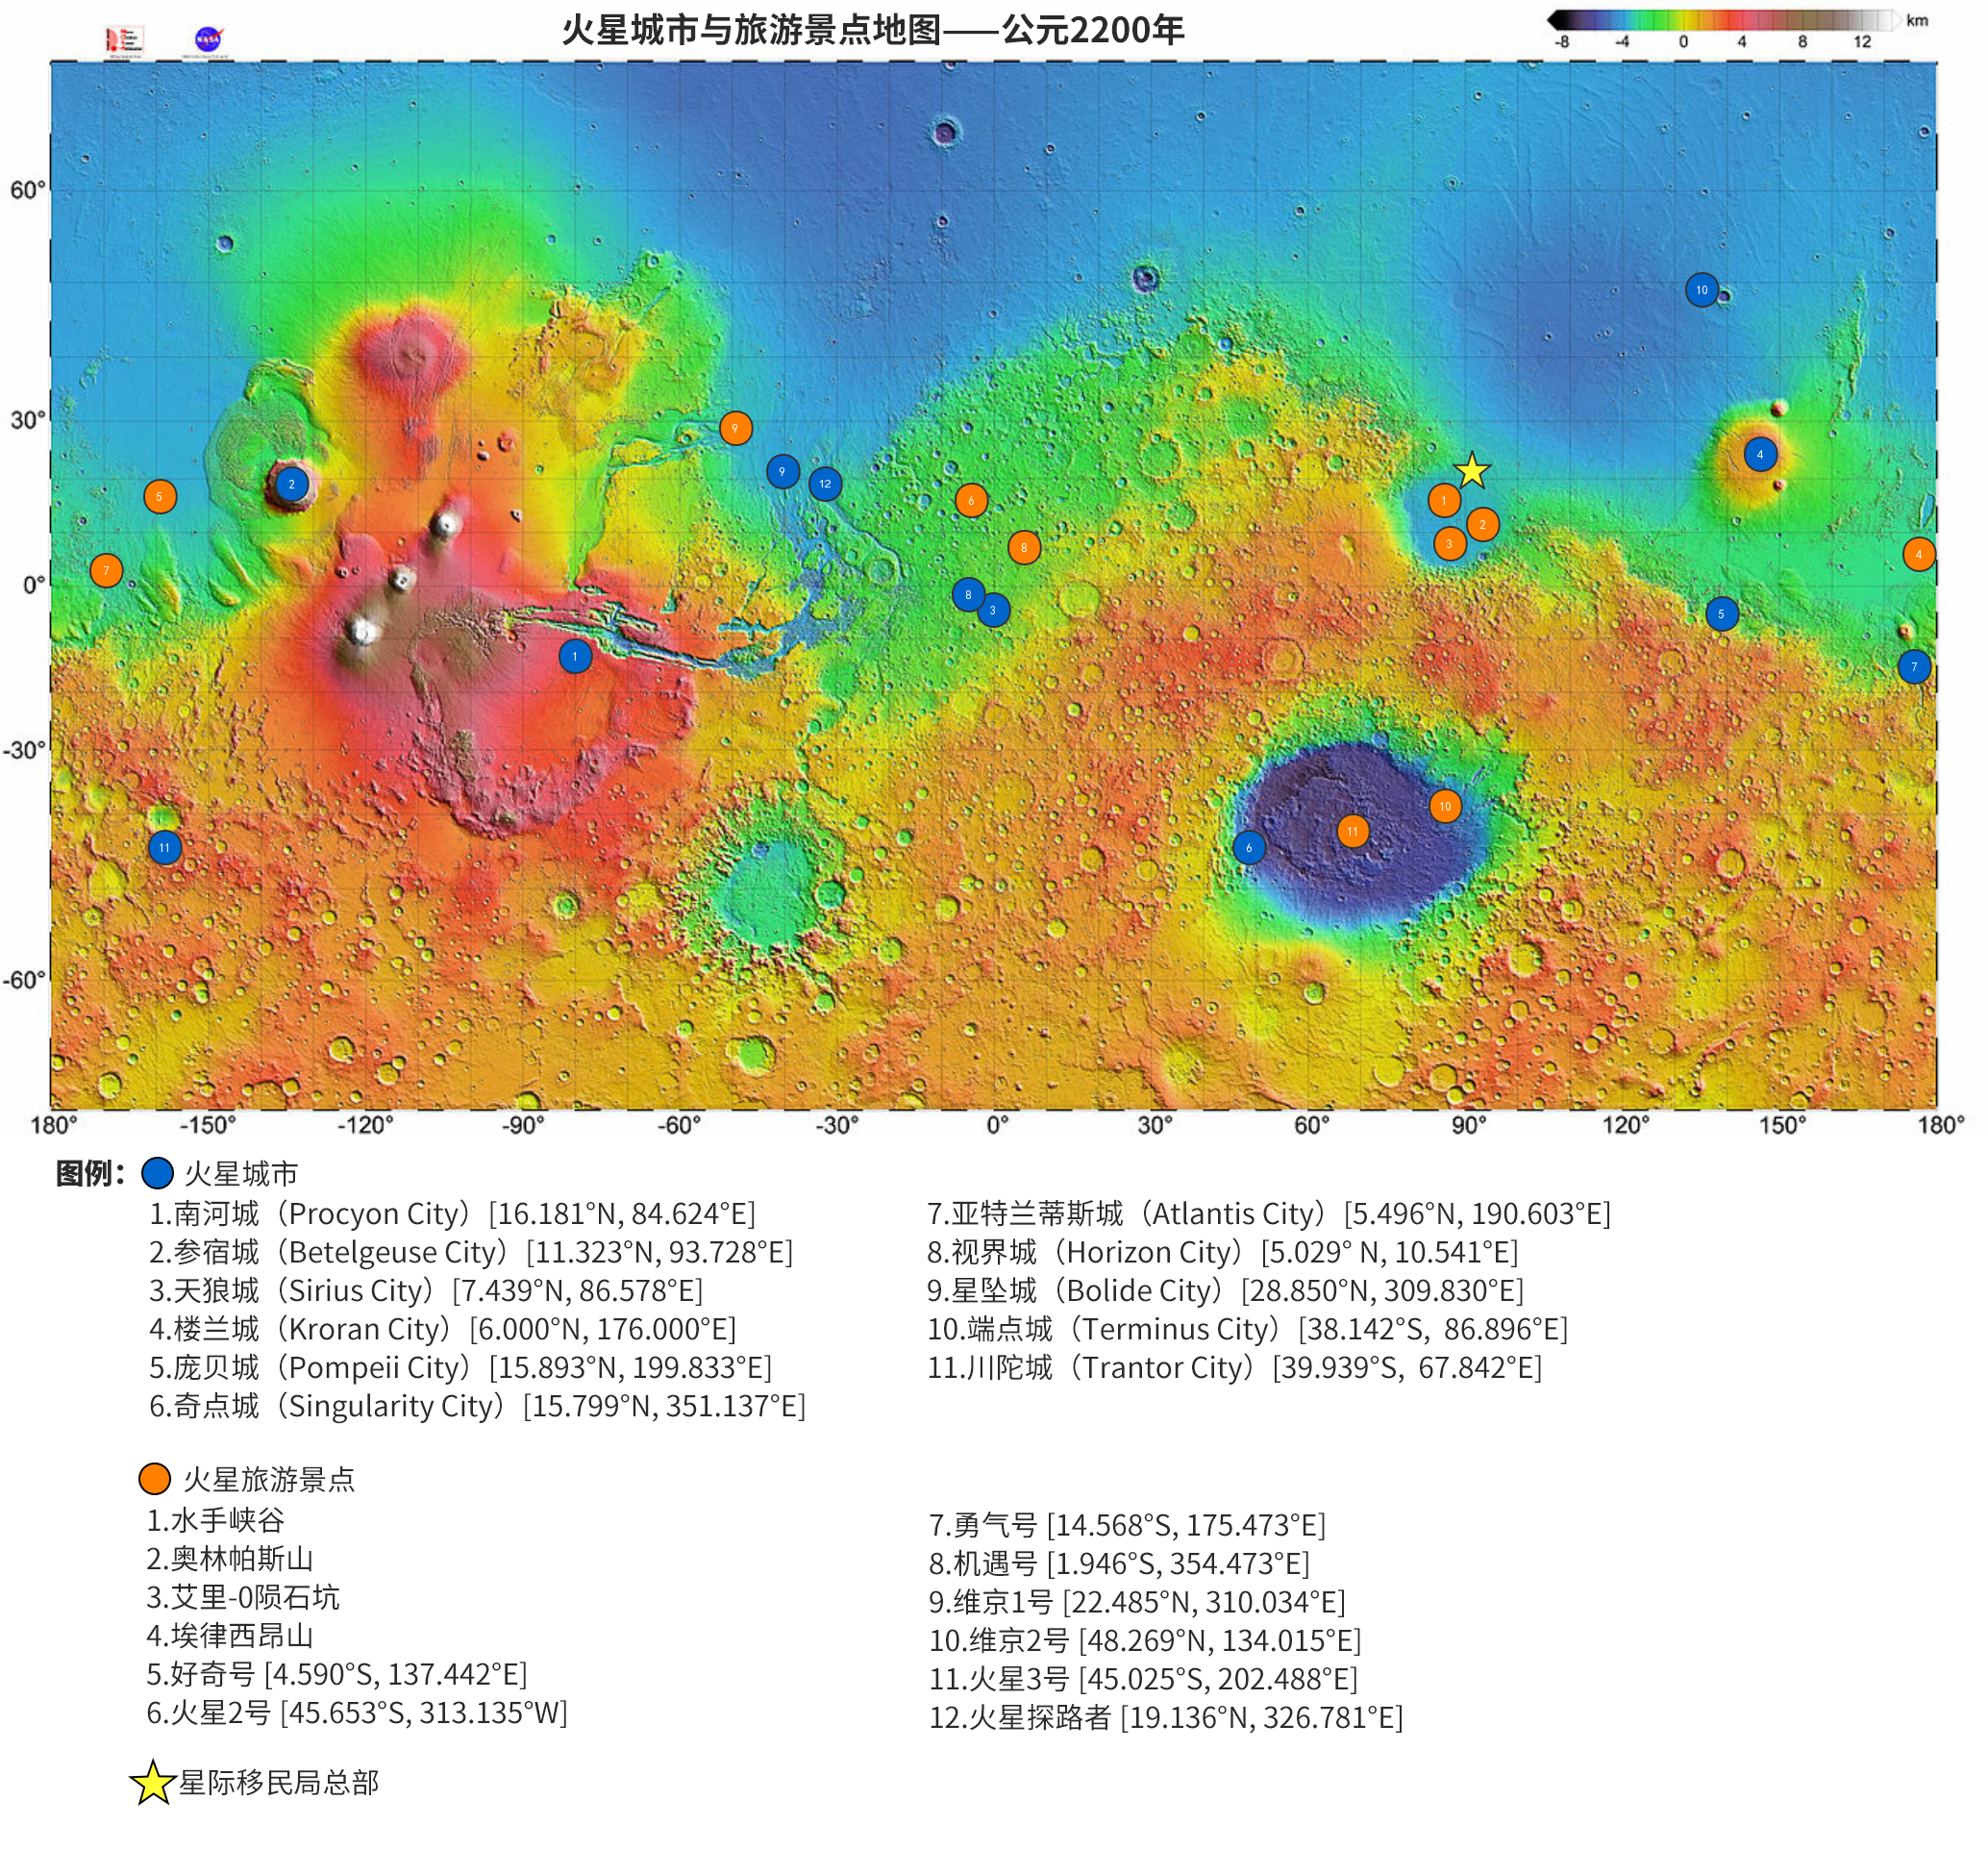
\includegraphics{marsCities.png}
\caption{火星城市及旅游图。基于 \href{http://mola.gsfc.nasa.gov/images.html}{NASA MOLA} 地图制作。在 Google Mars 中导入 此 KMZ 文件 ,可以观察火星城市具体位置。}\end{figure}

\begin{notice}{note}{火星城市历史}

火星城市发展历史请参阅 \href{http://interimm.org/InterImmBook/cities.html}{城市} 。
\end{notice}


\section{城市}
\label{cities::doc}\label{cities:id1}

\subsection{火星城市发展历史}
\label{cities:id2}
推进技术发展起来之后,从地球到火星变得方便快捷,许多火星前哨战和基地被建立了起来。许多实力较强的势力最终能够将基地发展成为真正的火星城市。然而后来热潮过后,加上经济危机的影响,这种分散的“圈地运动”几乎停止,演化成为大家围绕大型城市和基地扩展的竞争。

\begin{notice}{note}{火星前哨战、基地和城市}

火星前哨战是人数大于100人的聚集区,火星基地的要求为人数大于1000人,而火星城市是人数多于10000人的聚集区。
\end{notice}
\begin{figure}[htbp]
\centering
\capstart

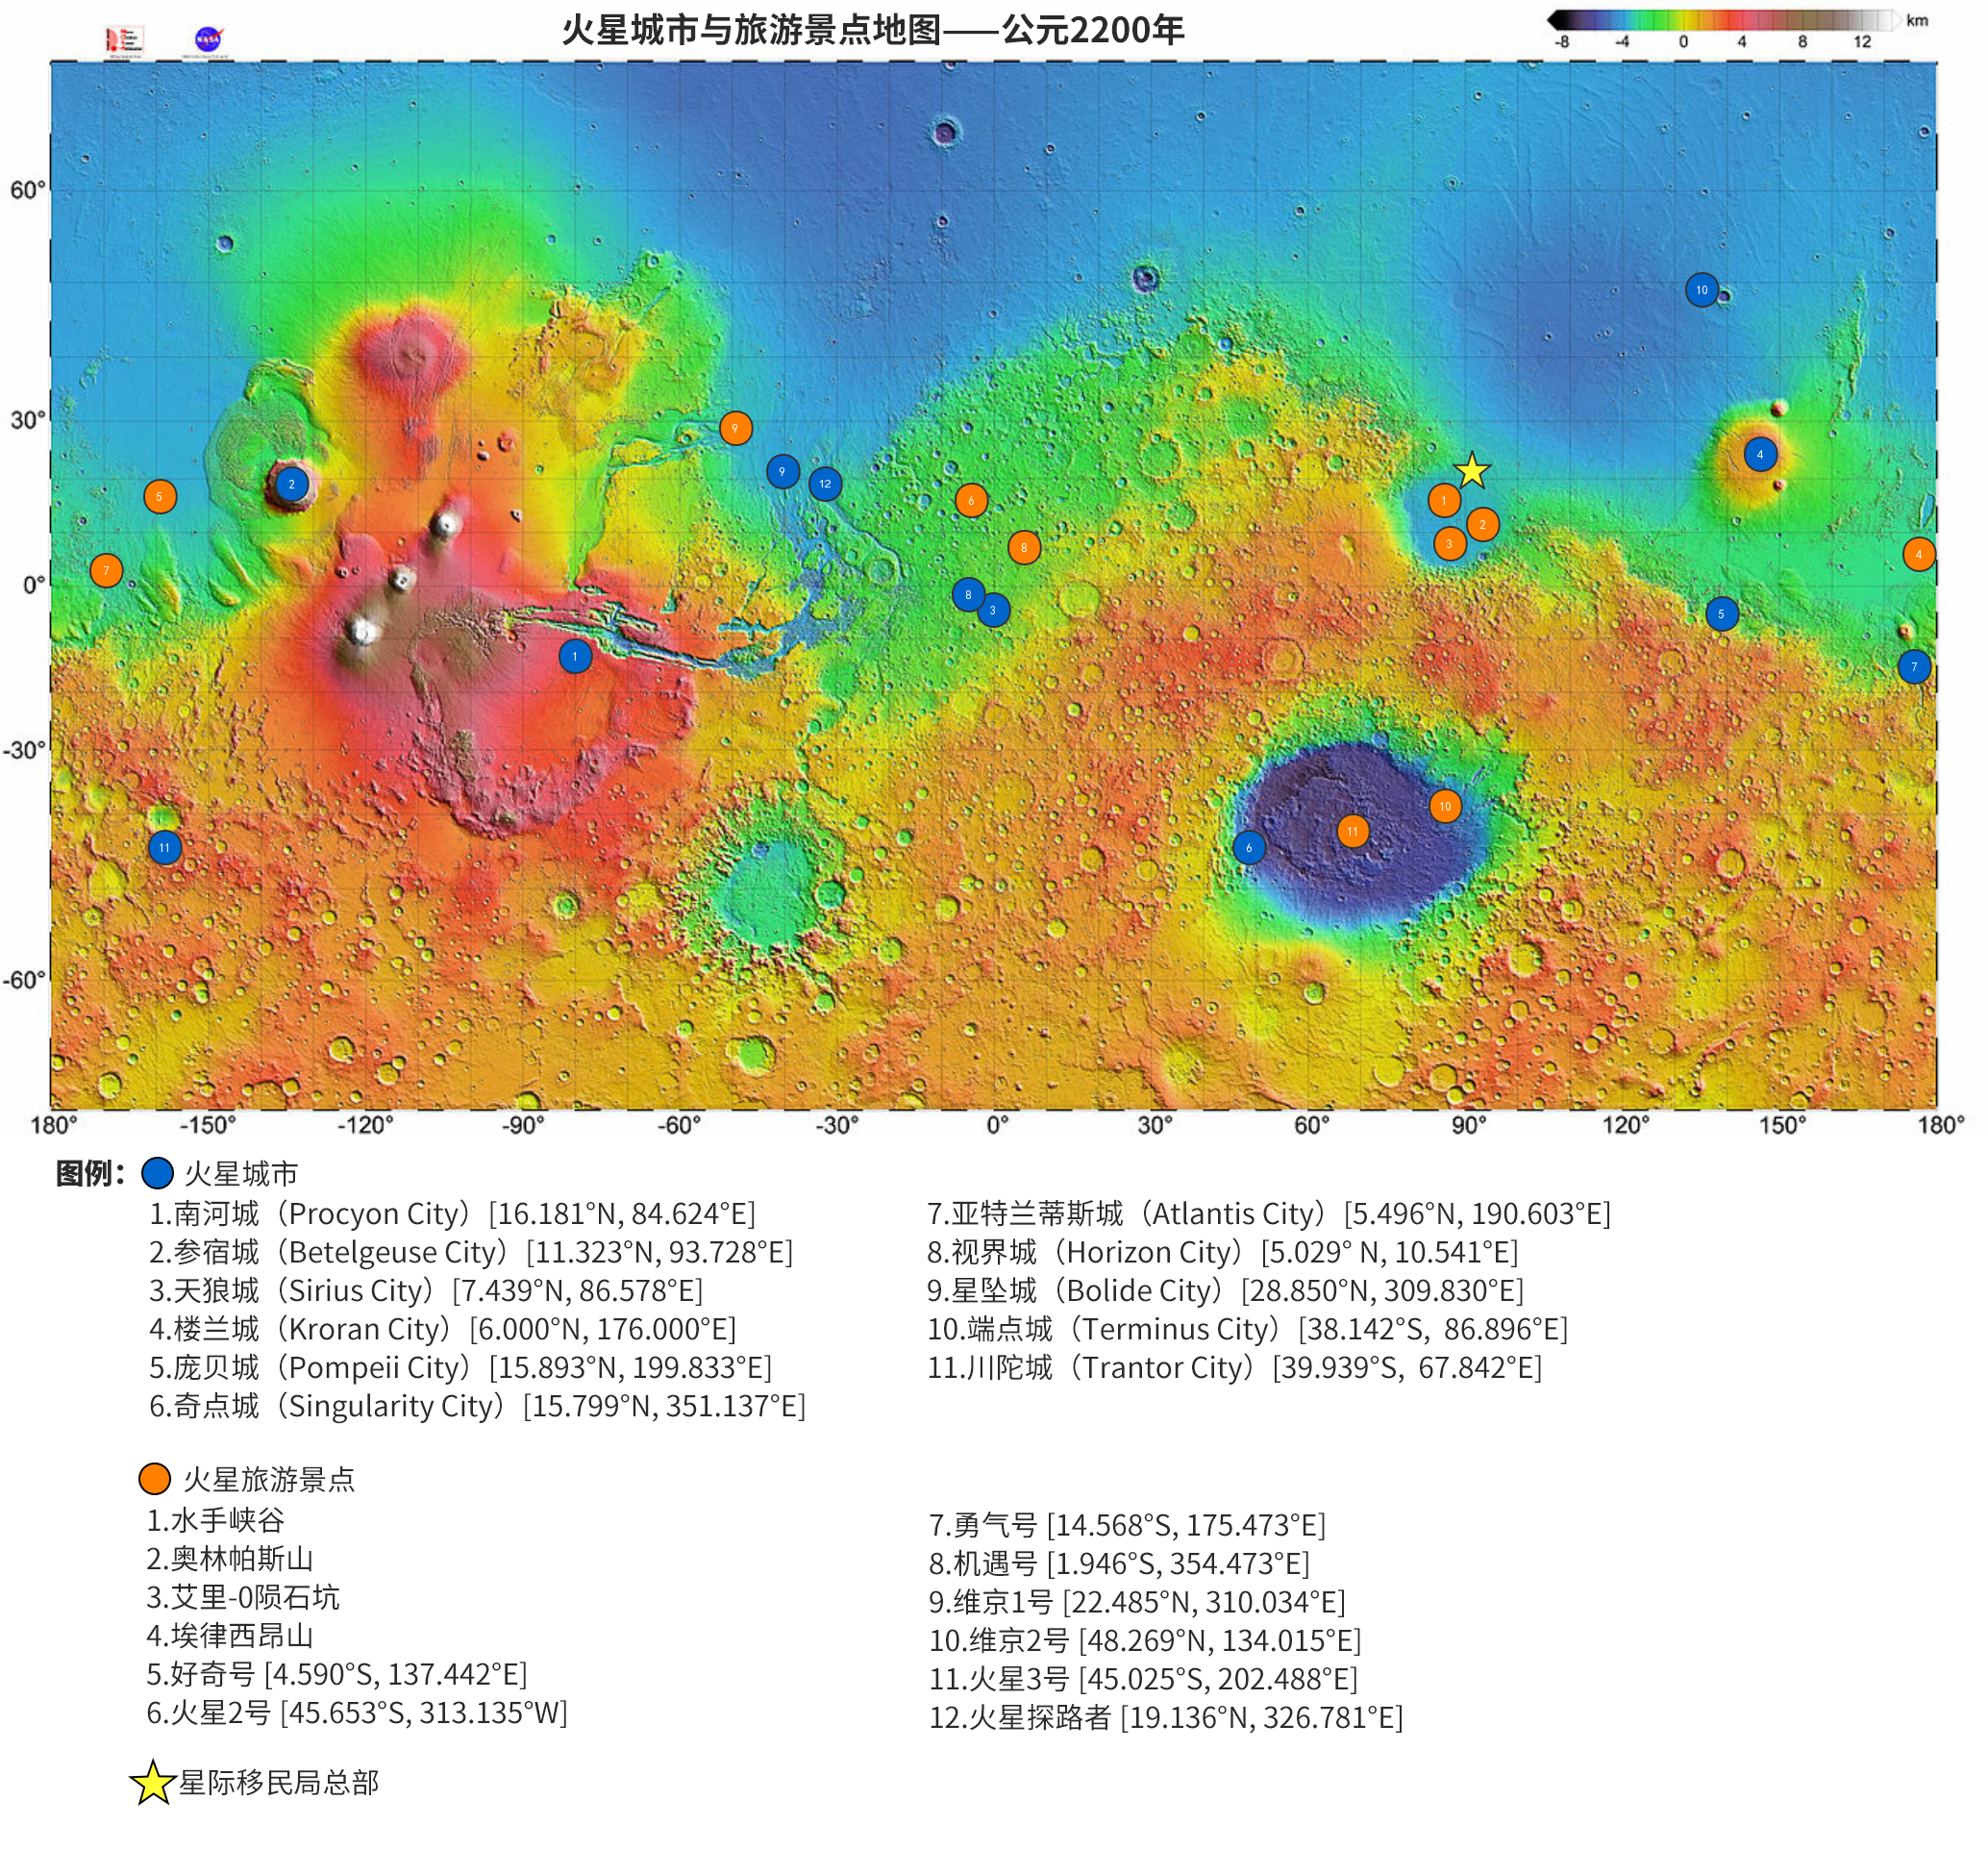
\includegraphics{marsCities.png}
\caption{火星城市及旅游图。基于 \href{http://mola.gsfc.nasa.gov/images.html}{NASA MOLA} 地图制作。在 Google Mars 中导入 此 KMZ 文件 ,可以观察火星城市具体位置。}\end{figure}

\index{伊希地城市圈}
\index{Isidis Metropolitan Area}

\subsubsection{伊希地城市圈}
\label{cities:index-1}\label{cities:id3}
自2070年第一个火星殖民地在伊希地平原建立后,随着殖民地规模的不断扩大,到22世纪初年逐渐发展到了地球上一座中等城市的规模,并被火星和地球上的人们称为“伊希地一号城”,简称一号城。

相比 IIA 当初提出的火星移民规划,一号城的建成速度和建成规模都远超预期。不过,在22世纪初的火星移民热潮时期,地球上的移民需求逐渐攀升,一号城已经无法继续应对逐渐涌入的移民人潮。因此,二号城、三号城的建设计划呼之欲出。

考虑到资源运输的便捷性,二号城和三号城的选址均位于伊希地平原。这两座城市建设过程中所使用的资源和源几乎全部来自于一号城。在两座新的城市建成后,新的移民和许多一号城的殖民者纷纷涌入,三座城市之间的交流与联系十分密切。22世纪20年代,火星上第一个繁荣的城市圈在伊希地逐渐形成。

\index{南河城}
\index{参宿城}
\index{天狼城}
\index{Procryon City}
\index{Betelgeuse City}
\index{Sirius City}
2123年2月17日,经过三地殖民者的全民公决,一、二、三号城以冬季大三角三颗星的名字命名,分别称为“南河城(Procyon City)”、“参宿城(Betelgeuse City)”、“天狼城(Sirius City)”。

\index{亚马逊城市圈}
\index{Amazonis Metropolitan Area}

\subsubsection{亚马逊城市圈}
\label{cities:id4}\label{cities:index-9}
在参宿和天狼的建设时期,IIA 就已经开始酝酿开发火星上的各类资源。随着火星人口的快速攀升,许多年轻的探险者不满足仅仅居住于伊希地平原的三尺之地中,他们宁愿穷尽自己的青春岁月也想要览尽红色星球的奇观异貌,即便是离开条件优越的火星城市,踏向未有人涉足过的生命禁区。

除此之外,火星考古及地质考察工作也在整个火星陆续展开,这些勘探者们实地采集了很多重要的数据,为资源勘探、火星远古生态的研究提供了宝贵的资料。

为了给探险者和勘探者提供支持,IIA 在火星的一些主要地点周围和前往这些地点的必经之路上设立了很多小型的补给站。这些补给站通常由三四个生活舱和几个存储舱构成,能够在这荒凉的火星上为过往的人提供休憩的场所,以及水、食物、能源和燃料的补给。截止22世纪中叶,这类补给站的数量已经达到了数百个之多。

埃律西昂山和奥林帕斯山是火星上最为热门的旅游及勘探地点之一。由于距伊希地较近,且路途十分平坦,往来于这两山一地的人较多,这一带补给站的规模也随之扩大。四号城和五号城正是由两个亚马逊平原的补给站慢慢发展起来的。

七号城的发展历史较四、五号城更晚。这里的地势较为复杂,并不平坦,不过由于富集的铁矿石资源和低纬度优势,这里发展成为了能源与矿业重镇,很多机械制造公司也将厂址选在七号城,不过也因此,七号城的居住环境和生活条件并不理想。

\index{楼兰城}
\index{庞贝城}
\index{亚特兰蒂斯城}
\index{Kroran City}
\index{Pompeii City}
\index{Atlantis City}
22世纪50年代,以四、五、七号城为核心的亚马逊城市圈初步建立,当地殖民者用地球古代的城邦为自己的城市命名,分别称为“楼兰城(Kroran City)”、“庞贝城(Pompeii City)”和“亚特兰蒂斯城(Atlantis City)”。

\index{子午线城市圈}
\index{Meridiani Metropolitan Area}

\subsubsection{子午线城市圈}
\label{cities:index-17}\label{cities:id5}
在七号城建立之前,一些火星本土公司就开始计划在火星的其他地方投资建造新的城市。不过因为资金及地理位置等原因,很多新建地并没有快速发展起来,只达到了火星基地的规模(1000 人以上,10000 人以下),甚至仅建成为了火星前哨站(100 人以上,1000 人以下)。

\index{火星地产开发}
\index{Mars Real Estate Industry}
\index{MREI}
由火星地产开发(Mars Real Estate Industry,简称 MREI)于 2139 年投资建设的六号城原本只是一所规模不大的地质考察站。随着资金的进入,许多建设资源从伊希地通过飞艇空运到六号城。为了吸引更多的人搬到六号城居住,MREI 在城市的便捷性和舒适性设计方面下足了功夫,也不惜巨资购买了一批十分罕见的地球珍惜动植物,将六号城打造成为火星上最为移居的城市之一。

\index{奇点城}
\index{Singularity City}
2145 年,在六号城正式落成的同时,MREI 将其命名为“奇点城(Singularity City)”,并向其他城市投送铺天盖地的商业广告。一些年事已高又小有积蓄的人被奇点安逸的生活条件吸引,在这里买下了 MREI 的不动产。

\index{视界城}
\index{Horizon City}
\index{视界星港}
\index{Horizon Starport}
就在奇点的人口不断上升的同时,2148 年,MREI 又开始在奇点的东南——子午线的另一侧建造另一座城市——视界城(Horizon City)这里原本是子午线高原惟一的一座小型星港,能够将质量不大的载荷送入近火轨道,也能够接收来自太空的货物。视界的商业开发模式和奇点相似,最后在2153年落成。“视界星港(Horizon Starport)”也建成为当时火星上最大的星港,许多往来的货物都在此转运。

由于 MREI 对六号城的商业开发,原本的地质考察站只能移至他处。九号城的前身正是搬迁到克里斯平原卡塞峡谷谷口的新考察站。作为火星上最大的 \href{http://en.wikipedia.org/wiki/Outflow\_channels}{外流水道} 之一,卡塞峡谷很可能是由艾彻斯谷的巨大洪水形成的。卡塞峡谷对于研究火星上的水文有重要价值。正因如此,IIA 对这所新考察站的建设给予了很大的支持,在短短几年内,考察站很快发展为一所规模较大的地质研究所,很多地质学家将自己的工作地点迁到这里。

\index{行星地质大学}
\index{Planetary Geology University}
\index{星坠城}
\index{Bolide City}
2065 年,行星地质大学(Planetary Geology University)在地质研究所的基础上落成,九号城也已经初具规模。2067年,经过全民公决,这座以教育、科研为主的城市被命名为星坠城(Bolide City)。子午线城市圈也就此形成。

\index{希腊城市圈}
\index{Hellas Metropolitan Area}

\subsubsection{希腊城市圈}
\label{cities:id7}\label{cities:index-32}
希腊平原的矿产非常丰富,加之此处的水资源也远比其他低纬度地区丰富,所以希腊平原一开始就有多个前哨战甚至基地。当地的第一个城市就是在一个前哨战的基础上成立的。

\index{川陀城}
\index{Trantor City}
\index{艾娃火星}
\index{Ava Mars Inc.}
艾娃火星公司{[}\#avamars{]}\_ 在当地成立前哨战的时候,很多前哨战已经发展成为了比较大的基地。然而艾娃火星公司与当地基地建立了良好的合作关系,并且与行星资源公司建立了合作,前哨战迅速发展成为基地规模。艾娃火星提出与其他机构的更加开放的合作关系,这个计划后来成为了火星*“川陀城”计划,于 2155 年开始整合建设。

\index{端点城}
\index{Terminus City}
川陀城正式开工之后第二年,即 2158 年,由星际移民局投资的在希腊平原边缘的城也开始建设。该城从开始建设就被命名为端点城,因为城市选址在希腊平原边缘,而开工时已经有希腊平原中心的川陀城在建。

端点城被设计为农业为主的城市。得益于技术的发展和大量资金的涌入,端点城的基本建设只花费了两年的时间。而更早开始的川陀城却在端点城建成之后一年才完工。由于完工更晚,川陀城在编号上成为第十一号城市,而端点城是第十号城市。

川陀城和端点城之间有着非常密切的合作,不仅仅在资源互惠上,在经济上甚至人口流动上,两个城市一开始就表现的非常友好。2068 年,两个城市决定开放更多的互惠资源,形成希腊城市圈。


\subsection{太空城市}
\label{cities:id8}
太空城市的出现,太空工业的推动起到了非常重要的作用。3D打印、大型太阳能板的发展,以及太空生产能力的增强,太空城的建造周期大大缩减。


\subsubsection{大型空间站}
\label{cities:id9}
2034 年,作为太空采矿业领跑者的行星资源公司与太空 3D 打印业的 Made in Space 公司启动了第一个 20 米直径的小型旋转圆环空间站计划。这是第一个太空生产的模型,环绕地球运行。2038 年,行星资源公司的 200 米直径、10 米宽度的旋转空间站工厂开始,同样是在近地轨道。空间站于 2040 年建成,并且进行了工作人员居住的测试。

这两个环形空间多方面指标都非常令人满意,成为后来大型空间站的模板。


\subsubsection{太空城市}
\label{cities:id10}
大型空间站运行稳定,激发了人们更加野心勃勃的计划:建造太空城市。第一个太空城市为了获得更大的生活空间,采取了圆筒形的设计。直径达到了 1000 米,然而考虑到稳定性的问题,轴长度设计了 500 米。这是一个两端封闭的圆筒形太空城市,使用多辐条来拉紧圆筒。同时辐条上安装有电梯快速到达太空城的其他地方。

第一个太空城的生活空间并不是特别理想,因此第二个太空城直径达到 2000 米,并且采用了双层结构,第一层直径为 1500 米,第一层并不是一个完整的圆筒,而是由三个六分之一圆筒的平台组成。整个空间站采用六组辐条结构,其中三组穿过第一层平台。


\section{职业}
\label{profession::doc}\label{profession:id1}
在火星移民兴起的背景下,许多新的职业应运而生。


\subsection{太空工程师}
\label{profession:id2}

\subsubsection{飞船驾驶员}
\label{profession:id3}
按照《太阳系和平开发与利用公法》(简称系法)中关于飞船驾驶的有关规定,货运飞船可在无人驾驶的情况下按照预定航线进行自主飞行,并由引航员进行远程跟踪与遥控。而对于载人飞船,为了保障乘客的安全,至少需要配备一名合格的飞船驾驶员。

随着地火航线及其他周边航线的开通,对于载人飞船的需求量逐年上升。此外,购买私人飞船也在富人圈子中也流行起来。不过,由于飞船的驾驶需要特定的训练和认证,很多人都不想花费太多的精力来取得飞船驾驶执照,而是选择聘请专业的飞船驾驶员。
\begin{figure}[htbp]
\centering

\includegraphics{290500.jpg}
\end{figure}

\index{太空捷运公司}
\index{Space Express Company}
\begin{notice}{note}{太空捷运公司}

UPI 旗下的 \textbf{太空捷运公司(Space Express Company)} 拥有数量众多的飞船驾驶员,还提供驾驶员培训服务。而飞船驾驶员的资格认证则必须前往星际移民局下属的 \textbf{星际运输中心轨道运输部资格认证处} 。
\end{notice}

基本上所有现役载人飞船的驾驶单元均设有识别装置,只有取得相关资质的飞船驾驶员才能够启动飞船。


\subsubsection{飞船检修员}
\label{profession:id4}
飞船市场越来越大,私人飞船也越来越多,特别是往返于火星表面和绕火轨道之间的私人飞船急剧增加,而飞船的定期检修需要专业的飞船检修员来完成。

\index{本尼公司}
\index{The Benny Company}
\begin{notice}{note}{本尼公司}

\textbf{本尼公司(The Benny Company)} 是第一家飞船检修公司,该公司一直到 23 世纪初都是拥有最多的店面和员工的飞船检修公司。在该行业刚刚起步的时候,飞船检修员特指飞船检修中指导大家进行检修的人员,对他们的电子、机械、推进等等各种专业知识要求非常高。伴随着技术的进步,飞船检修工具也变得非常容易操作,一艘小型飞船的检修一个人就可以完成,飞船检修员也不再特指检修小组组长,而是指那些操作检修机器的工作人员。
\end{notice}
\begin{figure}[htbp]
\centering

\includegraphics{330250.jpg}
\end{figure}


\subsubsection{飞船引航员}
\label{profession:id5}
货运飞船通常不需要配备飞船驾驶员,不过按照系法规定,在货运飞船进行起飞、降落、变轨等重要操作时,必须至少要有一名引航员进行监测和必要时的控制。在同一艘货运飞船航行的不同阶段,引航员通常会进行更换,更换依据“最短光秒”原则,这是为了将引航员与飞船间的控制时差降到最低。

对于地火货运航线,通常只需要地球、火星各一名引航员就足够了。而对于近地小行星航线,因为不可能在所有小行星矿场上都配备引航员,所以一般会在一些特殊的地方设立监测站,三个最大的监测站分布在地日 L3、L4、L5 点,其余的监测站分布在一些资源丰富、货运量大的小行星上。
\begin{figure}[htbp]
\centering

\includegraphics{800px-Lagrange_points.jpg}
\end{figure}


\subsubsection{重型机械操作员}
\label{profession:id6}
太空重型机械虽然大多实现自动化,但是某些机械依然需要人的控制,特别是体型庞大而笨重的重型机械。另外,对于小行星矿场这样的重型机械集中的地方,虽然自动化生产已经实现,但是值班员也必须在监控室实时监控,一旦出现故障,可以及时处理。

小行星采矿行业在发展的高峰时期,曾经使用过巨无霸挖掘机,这些挖掘机虽然可以进行自动化挖掘工作,但是在一些具体的细节上需要一些远程控制操作。在小型载人飞船真正发展起来之前,太空重型机械操作员大多是在地球、火星或者空间站中对机械进行遥控操作的。各种类型的太空机械的出现,也使得太空重型机械操作员越来越多。而后来的重型机械操作员,很多已经在机械的现场工作了。


\subsubsection{太空打印工程师}
\label{profession:id7}
自从第一次载人火星任务之后,3D 打印逐渐成为太空中的机械制造的主流方向。太空打印市场的兴起,带来了许多门槛较低的太空职业,太空打印工程师的市场需求越来越大,甚至出现了几种侧重点不同的太空打印工程师资格认证考试。

太空打印实际上是高度自动化的过程,然而模型设计、打印机维护以及程序维护等很多需要值守人员,太空打印工程师就是受过从设计到最后产出全面培训的人员。

\index{Made in Space}
\begin{notice}{note}{Made in Space}

Made in Space 是成立于载人登火之前(2010)的一家公司,他们是第一家在太空中直接制造产品的公司。在之后的登火热潮中,该公司的业务急剧增长,经济实力也越来越强大,开始赶超许多大型的地球上的 IT 公司。
\end{notice}


\subsubsection{轨道设计、规划与调度}
\label{profession:id8}
随着航天器、空间站和小行星工厂的增多,选择一条合适的太空航行轨道要考虑到发射窗口、燃料消耗、航行时间、飞行安全、运输成本等等诸多因素,这一切都属于轨道设计、规划与调度工作。


\subsubsection{太空垃圾清扫}
\label{profession:id9}
需要清扫的太空垃圾一般仅包括地球轨道与火星轨道报废的航天器,虽然转移轨道上也会有少量太空垃圾,但是由于星际空间过于广阔,转移航行时遭遇太空垃圾的几率比中“星球彩”特等奖的几率还小。

不过,地球与火星周围的情况却远没有这么乐观,如果不对太空垃圾进行清扫,轨道上运行的航天器将受到威胁。

\index{净伞科技}
\index{Clear Umbrella Technology}
\begin{notice}{note}{净伞科技}

\textbf{净伞科技(Clear Umbrella Technology)} 是太空垃圾清扫行业的起步者。最早的垃圾清扫采用轨道撒网、清扫器捕捉等方法,效率十分低下,并且无法清理尺寸较小的太空垃圾。
\begin{figure}[htbp]
\centering

\includegraphics{1280px-Sling-Sat_removing_space_debris.png}
\end{figure}

净伞科技最先采用“高能激光定向烧蚀”的技术来大规模地清理太空垃圾,在激光的作用下,尺寸较小的太空垃圾很快气化,而尺寸较大的太空垃圾在经过回收处理后,反而成了太空 3D 打印工厂的原料。
\end{notice}


\subsubsection{太空救援}
\label{profession:id10}
太空中有多个救援中心空间站,为了保障航行安全,在对飞船进行轨道设计与规划时,一般还要考虑到沿途救援中心的位置。

太空救援是高薪酬的职业,这并不是因为太空航行的事故率较高,而是因为救援的成本太大。从接到救援任务,到确定待救援飞船的位置,再到救援船到达事故地点并完成救援,一次救援工作的成本可能比一次航行的成本还要高。

太空救援一般分为人员救援与货物救援,救援的花费一般由相应的保险公司承担。对于人员救援来说,营救时间最为关键,要想快速接近事故飞船,就需要相当多的燃料,这些燃料比普通转移飞行所耗费的燃料要多得多。因此,救援中心的飞船都配备了最为强劲的引擎以及充足的燃料,以适应不同情况下的各种救援任务。


\subsection{太空运动}
\label{profession:id11}

\subsubsection{私人飞船驾驶教练}
\label{profession:id12}
由于驾驶飞船需要很多的技巧和知识,自己学习是非常困难而且危险的。飞船驾驶教练可以陪同练习并且传授驾驶的知识。


\subsubsection{太空健身教练}
\label{profession:id13}
太空环境的低重力等特点要求太空中的健身与地面的健身差异很大,而为了保持身体健康,太空中健身是必不可少的。太空健身教练就是专门为太空中生活的人民提供健身咨询和指导的健身教练。


\subsubsection{低重力游戏开发}
\label{profession:id14}
太空这类新的环境导致原来地球上大家喜欢的游戏不能正常的进行,所以有部分人开始专门为太空设计新的游戏,他们被称为低重力游戏开发专家。


\subsubsection{低重力格斗}
\label{profession:id15}
\index{太空综合格斗}
\index{SMMA}
\index{Space Mixed Martial Arts}
在低重力中,想要击倒一个人变得很困难,因为如果没有支撑,攻击方也会被推向相反方向。新的格斗技巧逐渐被开发出来,并且有些人成为了低重力格斗专家,另外也有些人专门表演低重力格斗。SMMA (Space Mixed Martial Arts),即太空综合格斗逐渐发展起来。每年的 SMMA 都会吸引大量的观众,各大企业也争相投资或投放广告。


\subsubsection{太空潜水}
\label{profession:id16}
太空潜水对于地球人来说是一项非常新奇的太空运动。太空潜水一般需要特殊的舱室,整个舱室内部都必须覆盖上一层防水材料。在失重的条件下,水的内部压强等于零,依靠着表面张力在舱室中形成分散的“水球”。太空潜水就是在这些大小不一的水球之间来回穿梭,在空间幻化无常的水体之中寻求不一样的体验。


\subsubsection{太空竞速}
\label{profession:id17}
类似于地球的方程式赛车,选手使用合乎规则的单人飞船参加竞速活动。太空竞速比赛一般在行星低轨道附近进行,比赛并没有固定的赛道,只有用无线电信标标示的起点与终点。比赛的内容即在最短的时间内从起点处到达终点处,整个过程必须手动驾驶,禁止使用自动导航系统。

尽管飞船都使用的是专业的竞速飞船,在对驾驶员的安全保障方面有所加强,这依然是一项高风险的运动。


\subsubsection{空间球}
\label{profession:id18}
地面上大多数的球类运动在太空中无法开展,不过,在低重力游戏开发师的奇思妙想之下,仍有一些深受喜爱的球类运动被搬到了太空,最风靡的并不是足球,篮球,而是“太空中的桌球”——空间球。

和大多数太空运动一样,空间球也需要特殊的舱室,通常是一个内部空间为球体的密封舱,舱内的六个方向各开有一个球洞。游戏规则和地球上的桌球类似,也是用白球撞击其他彩球进洞得分。不过,空间球却还要复杂很多,玩家在舱室内必须小心翼翼避免碰到球,架杆也更加困难。但相比其他运动,空间球所需空间小,更加易于推广,自然而然,空间球成为了太空中人们消遣娱乐的重要活动。


\subsection{太空农业}
\label{profession:id19}

\subsubsection{低重力园艺师}
\label{profession:id20}
低重力下的园艺与地球表面大有不同。由于生长素的分布不受重力影响,植物就无法根据重力来调整生长方向,导致植物生长相对杂乱。而低重力园艺就是利用失重的条件,通过光照、旋转产生离心力等方法使植物呈现出不同的形态。

\index{天际园公司}
\index{Heaven Garden}
\begin{notice}{note}{天际园公司}

最著名的低重力园艺作品当然是 \textbf{天际园公司(Heaven Garden)} 推出的“水晶之心”。在这件作品中,植物的营养液悬浮在失重环境中,白色的满天星以营养液为“中心”向外生长,最终形成一个立体的心形。天际园公司将培育完成的“水晶之心”密封固定在玻璃中,并运回地球进行销售。“水晶之心”深受地球人的喜爱,但是由于产量太少,一件小小的低重力园艺作品也价格不菲。从这以后,地球人也让开始逐渐了解低重力园艺师这个职业。天际园自然成为了女人心中的圣殿,男人心中的噩梦。
\end{notice}


\subsubsection{动植物培育员}
\label{profession:id21}
在火星前哨站的建设阶段,动植物培育员算是一个相当重要的工作。由于从地球运来的补给有限,而且还会受到发射窗口的限制,在火星上的动植物培育就成了关系到建设者生活质量甚至生命安全的重要工作。与从事基因改造等生物技术开发的研究人员所不同的是,动植物培育员并不要求很高的科研能力,时刻照料好自己所培育的东西就是他们工作的一切。当然,这也要求他们必须了解火星的环境对动植物生长带来的影响,必要时,培育员也会从专家那里得到技术指导。


\subsubsection{细胞培养员}
\label{profession:id22}
在太空中,由于失重的影响,动物的培育变得格外艰难,再加上空间所限,使得大规模的培育基本不可能。而对于植物,失重的环境也影响了它们的生长,产量因此下降。

不过,长期驻扎在空间站的宇航员可不满足于一日三餐的罐头食品,为了让他们也吃上新鲜的肉类,细胞培养员也被派驻到空间站中。

虽然通过细胞培养生产食物的技术已经相当成熟,并且相比地面的养殖与种植,细胞培养的生产成本更加低廉,更有利于大规模推广。然而,由于地球人对于这种人造食物天生的厌恶感,通过细胞培养技术生产食物在地球上遭到了大多数人的反对。

这种在地球上惨遭唾弃的技术却成了宇航员们的福音。为了让自己在太空中过得更加舒适一点,大部分宇航员都能接受食用培养食物。甚至有些宇航员在任务结束返回火星后,对培养食物念念不忘,反倒觉得真正的肉类索然无味。渐渐地,培养食物也在火星上悄然流行起来,红色星球对于细胞培养员的需求也越来越大。


\subsection{太空医疗}
\label{profession:id23}

\subsubsection{体检员}
\label{profession:id24}
为了防止外来细菌病毒的入侵,从其他地方回到火星或者地球,需要经过严格的体检才能通过海关。这正是海关体检员的工作。

另外,由于太空飞行对身体有特定的要求,体检员会对将要飞行的乘员进行检查,以确保飞行安全。


\subsubsection{太空护理师}
\label{profession:id25}
由于火星与地球在医疗条件上的差距,一些特殊的病人或者伤残人员需要转运到地球才能进行进一步的治疗。不过,转移航行的时间通常很长,要让病人平稳地度过转运期,不仅需要特别的医疗飞船,更需要专业的太空护理师照理病人的饮食起居。太空护理师也正是在这样的需求下出现的。

此外,一些有钱人为了自己的健康着想,也会雇佣个人太空护理师,来料理自己在飞船上的生活。


\subsubsection{营养师}
\label{profession:id26}
长期在太空中航行会对人的身体造成 \href{http://zh.wikipedia.org/zh-cn/\%E5\%A4\%AA\%E7\%A9\%BA\%E8\%88\%AA\%E8\%A1\%8C\%E5\%B0\%8D\%E4\%BA\%BA\%E9\%AB\%94\%E7\%9A\%84\%E5\%BD\%B1\%E9\%9F\%BF}{不利的影响} ,在低重力条件下,人体内的钙质容易流失,从而造成骨质疏松,肌肉无力等情况。除了每天进行锻炼,合理的营养补充也必不可少。

一般的商业载人飞船上通常会配备至少一名营养师,营养师与太空烹饪师相互合作,保障飞船上乘客的正常营养供应。此外,营养师还兼任了随船医生的职责,如果有乘客在航行途中出现不适,找营养师一般就能解决问题。如果情况较严重的话,就需要专业的医师进行远程协助才行。


\subsubsection{心理咨询师}
\label{profession:id28}
太空工作大多很孤单单调,而且需要经常在不同的环境(不同的重力、辐射、气压等)之间往返,很多人患上了一些心理疾病,而且常常会有一些与之前的心理疾病不同的表现,这促使了太空心理咨询的研究,并且有很多心理咨询师专业为太空环境中工作的人员服务。


\subsubsection{保育员}
\label{profession:id29}
火星并没有地球那样包裹全球的磁场,只有一些七零八落的微弱磁场,这使得火星上的辐射情况更为严重。在火星前哨站的建设阶段,星际移民局是禁止志愿者在火星上进行生育的,据说是考虑到了辐射对孕妇和胎儿可能造成的威胁。

在第一个殖民地建设的后期,火星上的首个保育站也随之落成。
保育站里配备了高级别的防辐射设施,生活条件也更为优越。在检测到怀孕之后,孕妇将会被第一时间转移到保育站中,由专业的保育员进行照管。在新生儿降生之后,保育员同样会负责照顾好婴儿。


\subsection{太空犯罪}
\label{profession:id30}

\subsubsection{太空走私者}
\label{profession:id31}
随着太空产业的发展,太阳系不同区域的资源和产品逐渐出现差异,太空走私者利用非法手段和廉价的运输方式,低价购入高价卖出,榨取高额的利润。

除了独自行动的走私者,还有很多走私者联合起来,形成了所谓的走私者联盟。他们相互袒护,共享部分利益,甚至利用一些空壳公司来牟取暴利。

\index{柳杉木业}
\index{Cryptomeria Wood}
\begin{notice}{note}{柳杉木业}

历史上有著名的“柳杉木业”走私案,涉及到的走私飞船多大两百多艘。\textbf{柳杉木业(Cryptomeria Wood)} 表面从事的是木制品行业,其中木制奢侈品是该公司最大的正当收入来源。为了谋取暴利,柳杉木业利用太空木质奢侈品的运输链,进行各种产品的走私活动,其中甚至涉及到大宗的致幻剂交易。最终被媒体披露,这些非法走私才进入公众视野,柳杉木业也最终得到了应有的惩罚。
\end{notice}

太空走私逐渐成为一条非常庞大的产业链,走私者使用的工具、飞船、伪造的证明文件等等,都用专门的供给商。


\subsubsection{太空大盗}
\label{profession:id32}
由于大多数常规飞船都有确定的航线,这使得太空大盗能够在合适的地点来盗窃或抢劫飞船的货物。

\index{黑色漩涡}
\index{Black Whirlpool}
\begin{notice}{note}{黑色漩涡}

在常飞地球火星驾驶员中,流传着一个关于“黑色漩涡”的传说。有飞船在飞到一些偏远区域的时候,会有一些涂有黑色漩涡图样的飞船突然出现,然后货物就会莫名的丢失,货仓内壁也会留下黑色漩涡的标志。传说有位驾驶员在货仓目睹了正在投到货物的盗贼,他们的宇航服上也有黑色漩涡的标志,这位宇航员躲在维修室没有被发现,所以才活了下来。这些太空大盗不仅仅偷窃,还会抢劫和杀人。他们所盗窃的飞船都不会留下任何影像和音频记录,这些飞船的日志系统无一例外的失灵了。

因为这些传说的原因,“黑色漩涡”成为太空大盗的代表标志。一直无法确定的是,“黑色漩涡”是一个组织,还是很多组织公用的标志。当然,另外有些亲身经历过被盗事件的驾驶员说,那不是一个黑色的漩涡,而是一个黑色的棒棒糖的样子。
\end{notice}


\subsection{太空服务}
\label{profession:id33}

\subsubsection{太空烹饪师}
\label{profession:id34}
低重力和低压下人的嗅觉和味觉会受到影响。太空烹饪师通过特殊的调料和食材,结合特定的方法,制作适合在太空中吃的食物,而一般的厨师使用地球的烹饪方法做出的食物在太空吃起来平淡无味。太空烹饪师无疑拯救了那些长期在这类环境中生活的人。


\subsubsection{火星/太空丧葬}
\label{profession:id35}
很多人相信人死后,太空才是最合适的归宿。因此太空殡仪服务也一度流行起来。另外,不少人也在遗嘱中说明要埋葬在火星的愿望。

火星/太空丧葬有多种多样的服务,包括太空坟场,太空漂流,火星坟场,火星高山葬,轨道墓碑等等。

太空丧葬是一个高收入行业,这点也吸引了不少投资公司投资相应的创业项目。

\index{世外天堂公司}
\index{Outer Heaven}
\begin{notice}{note}{世外天堂公司}

\textbf{世外天堂(Outer Heaven)} 就是一家著名的提供太空丧葬服务的公司。该公司运营了多家坟场,他们分布在太空轨道、火星、行星卫星和小行星上。比较著名的包括第四和第五拉格朗日点上的两片巨大的坟场,以及小行星坟场。他们提供了单个太空墓碑独占一颗小行星的服务,但是需要高昂的服务费用。
\end{notice}


\subsubsection{太空特殊服务}
\label{profession:id36}
太空特殊服务主要指太空性服务,该行业只在指定的地区合法,但是有很多非法经营,由于机动性好,非法经营很难完全被查处。特殊服务业主要是由联合国的 Space Prostitution Information Office 来管理,但是实际上的管理是联合国聘请其他机构或公司的人员来执行的。


\subsection{太空旅游}
\label{profession:id37}

\subsubsection{太空导游}
\label{profession:id38}
太空导游大致分为两种,一种是景点聘请的景点导游,这种导游入门门槛低,薪水也低。另一种是私人导游,这类导游通常具备多种技能,除了导游所需要的知识和技能外,通常持有非常高等级的飞船驾驶证,甚至也有各种急救等医疗技能和格斗术,通常受聘于富豪和名人,专门为他们提供导游服务。


\subsubsection{旅游景点勘探员}
\label{profession:id39}
由于很多地点尚未开发,并且荒无人烟,而新兴的飞行器使得交通成本变得低廉,旅游公司开始四处寻觅潜在的旅游景点。旅游景点勘探员在这种背景下应运而生。

勘探员需要按照一定的计划来勘探一片区域,找出潜在的旅游景点,并且撰写评估报告。评估报告中会详细描述该潜在景点的特色,可能的开发形式和可行性,以及潜在游客评估。可见从事此行业需要灵活的思维。


\subsection{太空商业}
\label{profession:id40}

\subsubsection{太空古董物件拍卖师}
\label{profession:id41}
很多地球人喜欢收集火星的古岩石、古旧的火星探测器等等带有火星意味的古物。火星古董拍卖师会对这些物品进行估价并且按照合法合理程序举办拍卖活动。

\index{天圆地方公司}
\index{Space Sphere}
\begin{notice}{note}{天圆地方公司}

Space Sphere ,即天圆地方公司,是第一家从事太空物件拍卖的公司,其旗下多名顶级拍卖师。但是在此之前,已经有很多个人在从事这个行业。尤其是将火星古董物件拍卖给地球上的某些收藏家。
\end{notice}


\subsection{太空艺术}
\label{profession:id42}

\subsubsection{太空画家}
\label{profession:id43}
在太空时代,新的绘画派别急速涌现,太空虚无主义、太空写实主义等等与太空相关的绘画派别变得越来越热门。与太空时代之前的太空绘画不同,太空画家所作的画,不仅仅是绘制太空,更是用来表达太空的精神。太空画家常常乘坐飞船去太空体验太空的味道,然后将从太空获得的灵感展现在作品中。其中太空写实主义绘画一直是最受欢迎的绘画,这类绘画真实的描绘了太空和其他天体上的情景。

在移民火星初期,太空虚无主义绘画发展到了一个高峰。这部分画家通过各种不同的技巧和技术辅助,来表现太空时代人类的迷茫。这些画家的作品大多带有非常浓郁的哲学意味,极力表达太空只是一个虚无的符号,而人类只是这个符号的一个细微到看不清的组成部分。广袤的太空强化了很多太空画家心中人生甚至人类无意义的虚无主义哲学。


\subsubsection{太空音乐人}
\label{profession:id44}
太空主题的音乐中,朋克音乐和死亡金属占了很大的部分。太空音乐以金属乐的发展作为起点,很多都涉及到太空的虚无、剧烈的死亡、爆炸的太空船等等。但是后来太空朋克逐渐在流行乐坛占了上风,与二十世纪的朋克文化的类似,太空朋克音乐也是标新立异,与传统划分界限。然而太空朋克音乐并没有持续非常长久。之后的太空音乐进入百花争艳的状态。

从事太空音乐职业中的自由音乐人的比例很高,他们从不跟任何公司签约,坚持独立制作。当然,大多还是职业乐队、职业作曲和职业作词。
\begin{quote}

\emph{Hit You Hard} 是一支著名的太空金属乐队,虽然从名字看来并不是特别像一支死亡金属的乐队,但是他们的音乐确实足够接近死亡金属。然而这支乐队的主唱却因为谋杀(将服务生扔进气闸,抛入太空)而入狱,终结了乐队在太空金属乐中独领风骚的地位。

太空朋克音乐并没有出现一支乐队独大的情况,流行榜不断被新的乐队刷新,然而这其中不得不提到 \emph{Down The Spaceship},因为这是一支诞生在太空船修理店的太空朋克乐队。所有的成员全部都是飞船检修员,他们的歌曲中也常常使用很多飞船检修的专业词汇,可谓独树一格。

太空音乐史上并没有出现新的大型的唱片公司。在职业音乐领域,依旧是太空时代之前的几家公司主导流行音乐的发展。但是他们却受到不少独立音乐人的冲击。
\end{quote}


\subsection{其他}
\label{profession:id45}

\subsubsection{外交人员}
\label{profession:id46}
星际移民局机构在地球多地设有办事处,因此需要外交人员来与地球沟通。这些外交人员就像地球上不同国家之间的使节一样,受到驻地尊重和保护。


\subsubsection{太空安保}
\label{profession:id47}
由于太空犯罪的出现,不得不设立太空安保人员来维持航线密集区以及人口密集的空间站、开发区等地的安全。


\subsubsection{太空律师}
\label{profession:id48}
人类在外太空开展的一切活动均应当在《太阳系和平开发与利用公法》的规范下进行,太空犯罪的特殊性要求从业律师具备更广泛的知识,因此太空律师逐渐成为一个新的职业。


\subsubsection{档案管理员}
\label{profession:id49}
几乎所有的机构都设有自己的档案馆,用来整理记录机构相关的档案。由于太空合作非常广泛,因此档案馆员之间需要非常频繁的交流才能完成一份优质完整的档案。


\section{科技}
\label{tech::doc}\label{tech:id1}
这是星际移民之书的科技部分。这一部分讲述了星际移民的相关科技。

星际移民对技术的要求很高,所涉及到的内容包括但不限于:
\begin{itemize}
\item {} 
行星探测,

\item {} 
生态系统,

\item {} 
星际运输,

\item {} 
星际空间定位和通信。

\end{itemize}


\subsection{行星际通信}
\label{tech:id2}
行星际通信在人类探索太阳系一开始的时候就是极为重要的一个分支。在火星移民开始之后,更加需要可靠高效的行星际通信系统。


\subsubsection{行星际通信中继}
\label{tech:id3}
由于时常出现的太阳和其他行星的遮挡,行星际通信需要一个可靠的中继系统。星际通信公司首先建立起了太阳极轨道中继卫星。并且发展出了一套辅助中继卫星,例如行星间直接通信卫星等。
\begin{figure}[htbp]
\centering
\capstart

\includegraphics{solarRelaySat.png}
\caption{太阳极轨道中继卫星系统。只需要三颗卫星即可到达全太阳系中继的目的。}\end{figure}

\index{鸿雁通信}
\index{Home Range Communication}
太阳帆技术逐渐成熟之后,新兴的 Home Range 通信(鸿雁通信)研发了一条非开普勒轨道的中继系统。第一个测试是地球-火星通信系统,采用太阳帆来让卫星维持在火星和地球上方的非开普勒轨道上。
\begin{figure}[htbp]
\centering
\capstart

\includegraphics{nonKeplerianRelaySat.png}
\caption{地球-火星非开普勒轨道中继卫星。来源:\href{http://strathprints.strath.ac.uk/25836/2/Macdonald\_M\_-\_strathprints\_-\_A\_novel\_interplanetary\_communications\_relay\_Aug\_2010.pdf}{A Novel Interplanetary Communications Relay}}\end{figure}


\subsection{太阳系内行星际运输}
\label{tech:id4}
\index{地火运输}

\subsubsection{地火运输}
\label{tech:earth2mars}\label{tech:id5}\label{tech:index-2}
\index{太空拖车}

\paragraph{太空拖车}
\label{tech:id6}\label{tech:index-3}
在第一个火星前哨站建立之后,UPI 的大宗货物运输是通过霍曼转移轨道进行的。由于当时在这种运输方式上的经验比较丰富,此方式被使用了多年。后来被称为“太空海运”,由于运输周期长,被人戏称为“太空拖车”。
\begin{figure}[htbp]
\centering

\includegraphics{hohmannSystem.png}
\end{figure}

运输器采用了大量的太空集装箱式的货仓设计,扩展方便。在 ULA 加入到火星殖民地建设中来之后,这部分逐渐完全转交给 ULA 负责。


\paragraph{星际弹道捕获}
\label{tech:id7}
弹道捕获的最早使用可以追溯到二十世纪人类发射的月球探测器 \href{https://en.wikipedia.org/wiki/Low-energy\_transfer\#History}{Hiten} 。通过这种方式到达环绕火星的轨道所需要的能量要比霍曼转移轨道的能量要低,然而也需要更长的时间。这种运输方式更加节省燃料,也就意味着同样的燃料可以运送更多的货物。在传统化学火箭时代,这种轨道是一种比霍曼转移轨道还要价格低廉,因此也长期存在。甚至在热核火箭和离子推进技术兴起的时代,这种运输轨道也被许多不知名的小机构继续使用。

轨道在前期与霍曼转移类似,然而通过霍曼转移并非直接到达火星,而是到达火星轨道之内的某处,然后采用一个弹道捕获的轨道慢慢地与火星会和。
\begin{figure}[htbp]
\centering
\capstart

\includegraphics{BallisticCaptureTransferStructure0.png}
\caption{弹道捕获的星际转移轨道。从地球出发,到达火星轨道之内的某处 $x_c$ 。参考 \href{http://arxiv.org/abs/1410.8856}{arXiv:1410.8856} 。}\end{figure}
\begin{figure}[htbp]
\centering

\includegraphics{BallisticCaptureTransferStructure.png}
\end{figure}


\paragraph{快速合点运输}
\label{tech:id9}
飞船采用快速的合点轨道前往目的地。虽然这需要更多的燃料,但是对于一些需要快速运输而且贵重的货物来说,这是最佳选择。UPI 还在很多小行星设立中转站,负责从地球出发的飞船的安全和紧急补给。

\index{星际弹射系统}

\paragraph{星际弹射系统}
\label{tech:index-4}\label{tech:id10}
小型物资的交换,需要比两年更小的周期。IIA 的研发部不得不考虑更加快捷的物质传输方式——星际弹射系统。

星际弹射系统的前身就是在 21 世纪 60 年代的电磁投射系统。在火星殖民开始前的准备中,IIA 已经将一个电磁投射器发射到了火星。在大规模的地面建设开始之后,工程船将绕火星轨道上的电磁投射器进行了改造和更新,建立了更加复杂精确的弹射系统,用来接收地球轨道或者小行星矿场直接弹射过来的物资。经过严密的计算之后,地球轨道上或者位于小行星矿场的的弹射系统会将物资弹出,经由一条较快的路径到达火星,轨道修正由货仓上的离子引擎完成。物资到达火星轨道后,位于火星轨道的弹射系统将为物资减速,进一步空降到地面殖民地。为了全程追踪,每个包裹都会装有唯一标识的无线电信号源。

\index{星际快车}
这类弹射系统后来演化为轨道加速器,也就是火星大规模移民的主要交通方式,被称为 \textbf{星际快车} 。


\paragraph{持续推进轨道}
\label{tech:id11}
在太阳帆、离子推进和热核火箭兴起之后,地球-火星之间有了快速安全的航线。得益于新的推进技术的发展,这种轨道采用了更加直接的方案飞往目标行星。
\begin{figure}[htbp]
\centering
\capstart

\includegraphics{ionThrustTrajectory.png}
\caption{地球和火星之间的快速航线。整个过程中发动机几乎全程开机,直接飞往目标行星。参考: \href{http://www.adastrarocket.com/Andrew-SPESIF-2011.pdf}{VASIMR Human Mission to Mars} 。}\end{figure}

\index{横跨轨道加速器}
\index{Transorbital Accelerator}

\subsubsection{横跨轨道加速器(TOA)}
\label{tech:toa}\label{tech:index-7}
在太阳系内行星之间的运输是通过横跨轨道终端来实现的。横跨轨道终端是一个加速器,可以将飞船在短时间内加速到行星际飞行的速度,这样节省了飞船自身的燃料,对于小型飞船来说,这是非常有效的方式。

例如,星际移民局总部在火星,常常需要快速的在地球和火星之间飞行,对于小型飞船来说,这是非常困难的,所以星际移民局在火星和地球分别建立了横向轨道跳跃装置。

小型飞船通过在火星的终端进行加速,可以达到非常高的速度,这样就可以迅速离开火星飞往地球,经过路途中的几个路径修正和最终靠近地球的减速终端,小型飞船就可以在不消耗自身燃料的情况下快速飞往地球。


\subsection{星际飞船}
\label{tech:id12}
在星际移民早期,主要使用的是化学火箭。后来由于核动力等离子火箭的大量使用,移民的成本大大降低,自由移民也开始大量出现。之后,曲率推进的大量生产,是的曲速飞船成为太阳系外移民的主要工具。


\subsubsection{离子火箭}
\label{tech:id13}
离子火箭是利用高压电场将电离后的物质加速并高速喷出来产生推动力的。
\begin{figure}[htbp]
\centering
\capstart
\caption{离子推进}\end{figure}

带电的离子在高压电场作用下,可以达到非常高是速度,从而将火箭推向相反的方向。由于离子火箭可以稳定的持续加速,所以适合远距离航行。

\begin{notice}{note}{扩展阅读}
\begin{enumerate}
\item {} 
\href{http://www.nasa.gov/centers/glenn/about/fs21grc.html}{Ion Propulson @ NASA}

\item {} 
\href{https://en.wikipedia.org/wiki/Ion\_thruster}{Ion Thruster @ Wikipedia}

\item {} 
早在二十世纪初,NASA 曾经对整个离子推进做过评估
\begin{figure}[htbp]
\centering
\end{figure}

\end{enumerate}
\end{notice}


\subsubsection{曲率飞船}
\label{tech:id14}
在恒星际移民的发展阶段大量使用的曲率引擎是 Markov-Alcubierre 引擎,是一种量子的 Alcubierre 引擎。曲率引擎(warp drive)的基本原理是通过弯曲时空来进行高速移动,因为要直接弯曲时空,所以所需要的能量非常大。Markov 在 Alcubierre 引擎基础上使用了量子的内禀对称转动与四维时空的耦合大大降低了能耗。

\begin{notice}{note}{扩展阅读}
\begin{enumerate}
\item {} 
中文维基百科词条: \href{http://zh.wikipedia.org/wiki/\%E6\%9B\%B2\%E9\%80\%9F\%E5\%BC\%95\%E6\%93\%8E\#.E6.9B.B2.E9.80.9F.E9.80.9F.E5.BA.A6}{曲率引擎}

\item {} 
Alcubierre drive, wikipedia 词条: \href{http://en.wikipedia.org/wiki/Alcubierre\_drive}{Alcubierre Drive}

\end{enumerate}
\end{notice}


\subsection{恒星际运输}
\label{tech:id16}
\index{Krasnikov Tube}
恒星际运输的主要工具是 Krasnikov Tube,是一种时空的扭曲,可以通过管道来进行几乎瞬间的移动。但是管道的建造是需要通过飞船来“铺设”(扭曲时空),所以不想 Markov-Alcubierre 引擎的飞船一样可以飞往任意地方。不过 Krasnikov Tube 的优点是,只需要一次建造,之后多次重复使用,可以运送大量货物而不需要消耗很多能量,所以这种管道成为了恒星际运输的一种主要手段。
\begin{figure}[htbp]
\centering
\capstart
\caption{Krasnikov}\end{figure}

\begin{notice}{note}{扩展阅读}

\href{https://en.wikipedia.org/wiki/Krasnikov\_tube}{Wikipedia: Krasnikov Tube}
\end{notice}


\subsection{推进技术}
\label{tech:id17}
相关的推进技术除了现在常用的曲率推进之外,还有另外一些可以使用的推进技术。


\subsubsection{离子推进}
\label{tech:id18}
离子推进技术最早是由 Konstantin E. Tsiolkovsky 提出的。后来经过多人的发展(Robert H. Goddard, Ernst Stuhlinger, et al),成为一种实用的技术。

离子推进是利用被电磁场加速的带电粒子来产生推力的,而离子的最终速度对离子所带的电荷非常敏感。理论上来讲,电推动的情况下,同样的电压下,两倍的电荷几乎可以产生两倍的最终速度,也就是两倍的最终推力。

真正实用的离子推动有两大类:
\begin{enumerate}
\item {} 
电场推动;

\item {} 
电磁推动。

\end{enumerate}

\begin{notice}{note}{扩展阅读}
\begin{enumerate}
\item {} 
早在二十世纪初,NASA 曾经对整个离子推进做过评估
\begin{figure}[htbp]
\centering
\capstart
\caption{NASA 对推进技术的评估}\end{figure}

\end{enumerate}
\end{notice}

\index{曲率推进}
\index{Warp Drive}

\subsubsection{曲率推进}
\label{tech:id19}\label{tech:index-10}
曲率推进的主要的理论依据是广义相对论。Alcubierre 在二十世纪末提出了相关的理论,但是由于当时技术的限制,并不能对这类引擎进行试验。\footnote{
\href{http://arxiv.org/abs/gr-qc/0009013}{The warp drive: hyper-fast travel within general relativity} By Miguel Alcubierre.
}

Alcubierre 类推进的主要原理是产生一个时空泡泡,然后通过移动这个时空泡泡来移动飞船。其实就是通过操控 \textbf{空间} 来从一个地方移动到另一个地方的推进技术。
\begin{figure}[htbp]
\centering
\capstart
\caption{Alcubierre 推进}\end{figure}

如果把 \textbf{空间} 看作是橡皮膜,那么 warp drive 实际上就是在通过压缩前方的空间,拉伸后方的空间来「移动」的。就是说,我们想从 A 点出发到达 B 点,实际上我们只需要把飞船前方的空间压缩一下,全部拿到飞船的后方来,不就可以到达 B 点了么。有点像是,「我不过去,山会过来」。如果我们仅仅操控空间,而不影响时间,那么就太好了,我们可以从 A 以任意 \textbf{速度} 到达 B 地点,但是总会花费一点时间,因为我们把空间这块 \textbf{橡皮膜} 压缩起来或者伸展开去总需要一定的时间吧。

这种推进有种很大的优势,那就是飞船里面的人不会察觉到飞船移动状况的改变,因为局域的来看,我们实际上根本没动。

\begin{notice}{note}{曲率推进进阶}

Warp drive 可以达到很多倍的光速,而且时间膨胀效应很小,所以 warp drive 就是我们理想的载人航行器!

Miguel Alcubierre 提出了一种神秘的度规,这种度规恰好可以帮我们实现曲率推进,该度规就被称为 Alcubierre metric.

Alcubierre 度规是像是一个可以将飞船包裹起来的时空泡泡,泡泡内部还是正常的闵氏时空,然而这个时空泡泡却有一个时空剧烈变动的外壳。

Einstein 的场方程的两端可以分别是物质和时空,现在要做的只是设计一个合理的度规,然后按照上面的方程解出所需要的物质的分布和特性。

\textbf{推进器的重要参数 —— warp factor}

在 Star Trek 中,速度一直是使用 warp N 来表示的,warp 1 表示一倍光速,其他的按照
\begin{gather}
\begin{split}v=w^3c\end{split}\notag\\\begin{split}\end{split}\notag
\end{gather}
来计算,其中 $v$ 是闵氏时空中的测量速度,$c$ 是光速,$w$ 便是 warp factor(扭曲因子,wikipedia 上翻译为「曲率层级」,我觉得不够直观)。一开始的时候,开到 warp 5 就已经不得了了呢。

后来的剧集中,Okuda 更改了 warp factor 的定义,新的定义为 warp factor 为 1-9 时
\begin{gather}
\begin{split}v=w^{10/3}c\end{split}\notag\\\begin{split}\end{split}\notag
\end{gather}
而超过 9 就直接手绘了一条趋向无穷的曲线。到了 1995 年,有人给出了一个解析公式。下图是 \href{http://en.wikipedia.org/wiki/File:Warptable.gif}{wikipedia 中的新旧 warp factor 的对照表以及其能量需求等等量直接的关系} 。
\begin{figure}[htbp]
\centering
\capstart
\caption{Warp Factor}\end{figure}

\textbf{Alcubierre 度规}

Alcubierre 度规可以从 ADM 形式中猜出来,但是这个 Alcubierre 前辈已经写出来了,所以只需要把前辈的那个抄过来,
\begin{gather}
\begin{split}\mathrm ds^2 = -\mathrm dt^2+(\mathrm dx - v_s f(r_s)\mathrm dt)^2 + \mathrm dy^2 + \mathrm dz^2\end{split}\notag\\\begin{split}\end{split}\notag
\end{gather}
其中,
\begin{gather}
\begin{split}v_s=\mathrm dx_s/\mathrm dt\end{split}\notag\\\begin{split}\end{split}\notag
\end{gather}\begin{gather}
\begin{split}r_s=((x -x_s)^2 + y^2 + z^2)^{1/2}\end{split}\notag\\\begin{split}\end{split}\notag
\end{gather}\begin{gather}
\begin{split}f(r_s)=[\tanh(\sigma(r_s + R))-\tanh(\sigma(r_s - R))]/[2\tanh(\sigma R)]\end{split}\notag\\\begin{split}\end{split}\notag
\end{gather}
并且 $\sigma>0$,$R>0$。

怎么看这个度规呢,其实我们可以把飞船看做一个点,放在 $x_s$ 并让飞船的轨迹沿着 x 轴,然后 $r_s$ 可以看做是离开飞船的距离。然后我们看一下 $f(r_s)$ 这个函数的渐进行为。这个函数里面的 $\sigma$ 这个参数是用来调节 $\tanh$ 函数的陡峭程度的,同时也可以调节 $f(r_s)$ 这个函数的陡峭程度。下面我们看一个极端情况
\begin{gather}
\begin{split}\lim_{\sigma\rightarrow\infty} f(r_s)=\begin{cases} 1 & r_s\in [-R, R]\\0 & \text{其他.} \end{cases}\end{split}\notag\\\begin{split}\end{split}\notag
\end{gather}
也就是说,这是一个帽子函数。$\sigma$ 越大,这个帽子就越陡,而且中心越平坦。
实际上这保证了离飞船比较远的地方依然是闵氏时空。

有了 metric ,你就可以依据这个 metric 来计算所需要的物质了,然后就是如何得到这种物质并且给出特定的分布。在这之前,你需要检验一下这个度规是否真的满足我们的需求,对不对?

首先,检查一下飞船远处的时空状况。此时 $r_s$ 很大,度规退化成
\begin{gather}
\begin{split}\mathrm ds^2 = -\mathrm dt^2+\mathrm dx ^2 + \mathrm dy^2 + \mathrm dz^2\end{split}\notag\\\begin{split}\end{split}\notag
\end{gather}
恰是闵氏度规。

这样形象的来看,飞船就是被包裹在一个「时空蛋壳」里了。那么这个飞船可以行进多快呢?答案是想多快就多快。

因为飞船的移动完全依赖于 $v_s$ 的大小,我们通过调节这个参数的大小,就可以调节飞船在无穷远的人看来的「移动速度」。而且,Alcubierre 证明,这种移动没有时间上的膨胀效应,也就是说,在无穷远的人看来,如果飞船花了一天从 A 地点到达了 B 地点,那么飞船上的人也是同样这么认为的。
\end{notice}

\index{Krasnikov 通道}

\subsubsection{Krasnikov 通道}
\label{tech:krasnikov}\label{tech:index-11}
Krasnikov 通道是一种通过对时空进行修改从而达到一次修建多次使用的技术。\footnote{
\href{http://arxiv.org/abs/gr-qc/0207057}{The quantum inequalities do not forbid spacetime shortcuts} By S. Krasnikov.
}

通过修改时空来缩短两点之间的距离,使得时空形成一条稳定的管道,从而达到在两点之间快速移动的目的。

Krasnikov 仔细分析了管道的修建和因果关系,所以这类通道叫做 Krasnikov 通道。

\index{Heim 理论}

\subsubsection{Heim 理论}
\label{tech:heim}\label{tech:index-12}
在二十世纪 B. Heim 的几何化的场论为我们提供了描述两种不同于引力、电磁力、弱相互作用、强相互作用四种力的新的相互作用,并且提供了电磁相互作用和引力的更加紧密的联系的描述。这使得我们可以通过电磁力来操控引力。\footnote{
\href{http://www.hpcc-space.com/publications/documents/PrinciplesOfAdvancedSpacePropulsionAIAA-paper-2002-4094.pdf}{Physical principles of advanced space propulsion based on Heins' field theory}
}

Heim 的理论中,通过在不同的能量之间相互转换,既可以将飞船移动,不消耗推进剂也可以推进飞船。


\chapter{共同协作与内容协议}
\label{index:id5}
本项目是一个开源项目,欢迎加入到项目中来。点击边栏菜单中的 \emph{提交 BUG} 可以告诉我们书中的错别字、排版建议以及内容建议。

本书使用 CC BY-SA 协议共享。



\renewcommand{\indexname}{索引}
\printindex
\end{document}
